%%%%%%%%%%%%%%%%%%%%%%%%%%%%%%
% 	   美赛模板,正文部分		 %
%          PAPER.tex         %
%%%%%%%%%%%%%%%%%%%%%%%%%%%%%%
\documentclass[12pt]{article}

\usepackage[1915023]{easymcm}\problem{A}   % 控制号、题号和标题
\usepackage{palatino} % 这个是COMAP官方杂志的字体
\usepackage{epstopdf}

\title{A guide of raising Dragon}  % 标题

% 正文开始
\begin{document}
%%%%%%%%%%%%%%%%%%%%%%%%%%%%%%%%%%%%%%%%%
%%            请在此填写摘要            %%
%%%%%%%%%%%%%%%%%%%%%%%%%%%%%%%%%%%%%%%%%
\begin{abstract}\small
     When we read this problem at the first time, to associate Dragon with ecology  we came up with an idea, create a model centering energy. \\

    First, as fanatical fans of Game of thrones, we select "Mother of Dragons" as the reference object to estimate the Dragon's profile characteristics. Analogy birds, there is a equation shows relations between weight and wingspan. However, we found that this method is not suitable for two animals that are too much different in body size. Through access to information, we know that this equation don't fit creatures with too long wingspan. So we improve the model, and do test with Quetzalcoatlus. The director of this series said the adult Dragon is as heavy as a Boeing 747. Our model match this statement.\\

Second, in order to know energy consumed of Dragon,under our bold speculation, we set up a series of basic models for our futher study. To start with, we reference metabolism equation of land creature, base on this we correct the model. Besides, The result of the first edition fly process modelis too much bigger than expected. According to aerodynamics, considered the pressure difference between above and below the wings, we introduce a correction factor to account for the difference between the size of the wing disc and the actual tube of air displaced by the bird's wings, then pass verification.Then we build a spray flame process model,we assume a special organ for Dragon,and consider this process as flamethrower.Through calculate, we get the energy cost each spray.Now we get a realistic energy model.\\

Finally, we need to consider the energy model of the ecological system. In our opinion, if we want to emphasize the flow of energy in the ecosystem, we need to simplify the food chain and ecosystem energy structure. Then we gathered informations about climate and vegetation coverage of various regions. As a result, we draw figures about the relationship of weight,area,community. In an intuitive way, we shows that Dragon interact with different climate. It tells us the effection of the different regions with very different climates on growing Dragon etc.This just solved the problem of the interaction between the dragon and the ecological environment.\\\\\\\\

\textbf{Keyword: Energy, Aerodynamics, Ecosystem, Heat transfer, Bioenergy}
\end{abstract}



%%%%%%%%%%%%%%%%%%%%%%%%%%%%%%%%%%%%%%%%%%
% 如不理解以下部分中各命令的含义,请勿修改! %
%%%%%%%%%%%%%%%%%%%%%%%%%%%%%%%%%%%%%%%%%%

%---------以下生成sheet页----------
% 下面的语句可调整全文行距为标准值的0.6倍,请自行使用
%\renewcommand{\baselinestretch}{0.6}\normalsize
\maketitle  % 生成sheet页
\thispagestyle{empty}   % 不要页眉页脚和页码
\setcounter{page}{-100} % 此命令仅是为了避免页码重复报错,不要在意

%---------以下生成目录----------
\newpage
\tableofcontents
\thispagestyle{empty}   % 不要页眉页脚和页码
\newpage

%---------以下生成正文----------
\setlength\parskip{0.8\baselineskip}  % 调整段间距
\setcounter{page}{1}    % 从正文开始计页码
\pagestyle{fancy}		% 摘要请到ABSTRACT.tex中填写

\section{Introduction}
\subsection{Background} %Background
George R.R. Martin,a great fiction writer,shows us series of epic fantasy novels named A Song of Ice and Fire.In this novel,the "Mother of Dragons" Daenerys Targaryen raised three dragons.And the Dragons have their special characteristics.Therefore this amazing creature make us interesting in their lives,and we can't stop thinking about what will happened if these three dragons live today.


\subsection{Problem Restatement}%问题补充
Underpinning of the story,four major problems are discussed in this paper, which are:
\begin{itemize}
		\item The ecological impact and requirements of the dragons.
		\item The energy expenditures of the dragons, and what are their caloric intake requirements. 
		\item Required area to support the three dragons.
		\item A necessary size of community to support a dragon for varying levels of assistance that can be provided to the dragons.
\end{itemize}

\section{Assumptions and Symbol}
\subsection{Assumptions}%%假设
\begin{itemize}
\item Aquila chrysaetos is a suitable basic model.\\
Reason: (1)As one of the consequences of Galileo’s Square Cube Law, the relative power of animals decrease as a function of the increasing size of animals.$^{[2]}$ Further hampering the flying ability of large animals is the theoretical aerodynamic results showing that heavier objects need disproportionally more relative power than lighter flying objects.(2)In spite of Quetzalcoatlus is more similar with the Dragon in novel, there are too little available source to analysis today.

\item The combustible is liquid and store in a special organ of Dragon.\\
Reason: Dragon take a great amount energy to breathe fire.We found if it use gas to fire, it need a space bigger than himself. So we consider this creature have a special organ to store combustible liquid. Otherwise  when it want to spray flame, it will inhaling air and mix with atomized combustible in a air cavity.At most time the air cavity is contraction state, only when it prepare for spray flame, the air cavity is filled with mixed composition.

\item The Dragon is a kind of Warm-blooded animal. \\
Reason: Although the Dragon have a huge body, it still can act flexiable.Warm-blooded animal can maintain their body temperature at a higher level, their muscle contract faster, and Generally less fatigue.So we think it need a high enzyme activity to insure this.In addition, this temperature should not higher than 40 Celsius.

\item We found three typical filming locations of Game of Thrones, they are iceland,Tundra climate:an arctic region,morocoo,Tropical desert climate:an arid region,ireland,Temperate grassland climate:a warm temperate region.

\end{itemize}

\subsection{Symbol}%%物理量
The primary symbols used in this paper are listed in \textbf{Table \ref{tb:symbol}}.
\begin{table}[!htbp]
\begin{center}
\caption{Symbols}
\begin{tabular}{cl}
	\toprule
	\multicolumn{1}{m{3cm}}{\centering Symbol}
	&\multicolumn{1}{m{8cm}}{\centering Definition}\\
	\midrule
	$\alpha$ &Correction factor\\
	$P_{aero}$ &Aerodynamic power\\
	$P_{ind}$ &Induced power\\
	$P_{pro}$ &Profile power\\
	$P_{pro}^{'}$ &Corrected profile power\\
	$C_{Db}$ &Drag coefficient\\
	$\Gamma$ &Efficiency of assimilation\\
	$W_f$ & energy used for flight;\\
	$W_d$ & energy used for metabolic;\\
	$W_s$ & energy used for spray flame;\\
	$W_{in}$ & energy from food intake;\\
	$W_g$ & energy used for grow;\\
	$\rho$ & Density of air;\\
	$S_w$ & surface area of Dragon wingspan.\\
	$\gamma$ & Daily average radiant energy of light;\\
	$\beta$ & grassland coverage;\\
	\bottomrule
\end{tabular}\label{tb:symbol}
\end{center}
\end{table}

\section{The Mathematical Model of Huge dragon interact with Ecosystem}%%模型
\subsection{Characteristics of Dragon}%%龙的特点
\subsubsection{Weight of Dragon}%龙翼展重量模型
In order to calculate the weight of the Dragon we refered golden eagle's ratio of wing length to body weight.
\begin{equation}
	\frac{M_2}{L_2^3}=\frac{M_1}{L_1}.	%小型鸟类公式
\end{equation}
Where
\begin{itemize}
    \item M$_2$ is the weight of the animal(kg);
    \item L$_2$ is the wingspan of the animal(m);
    \item M$_1$ is the weight of child Dragon(kg);
    \item L$_2$ is the wingspan of child Dragon(m).
\end{itemize}
And soon we found this formula is not fit for bigger flighters with longer wingspan,so we improve this equation as follow:
\begin{equation}
	\frac{M_2}{L_2^3}=\left(\frac{M_1}{L_1}\right)^3.	%大型鸟类公式
\end{equation}

		\centerline{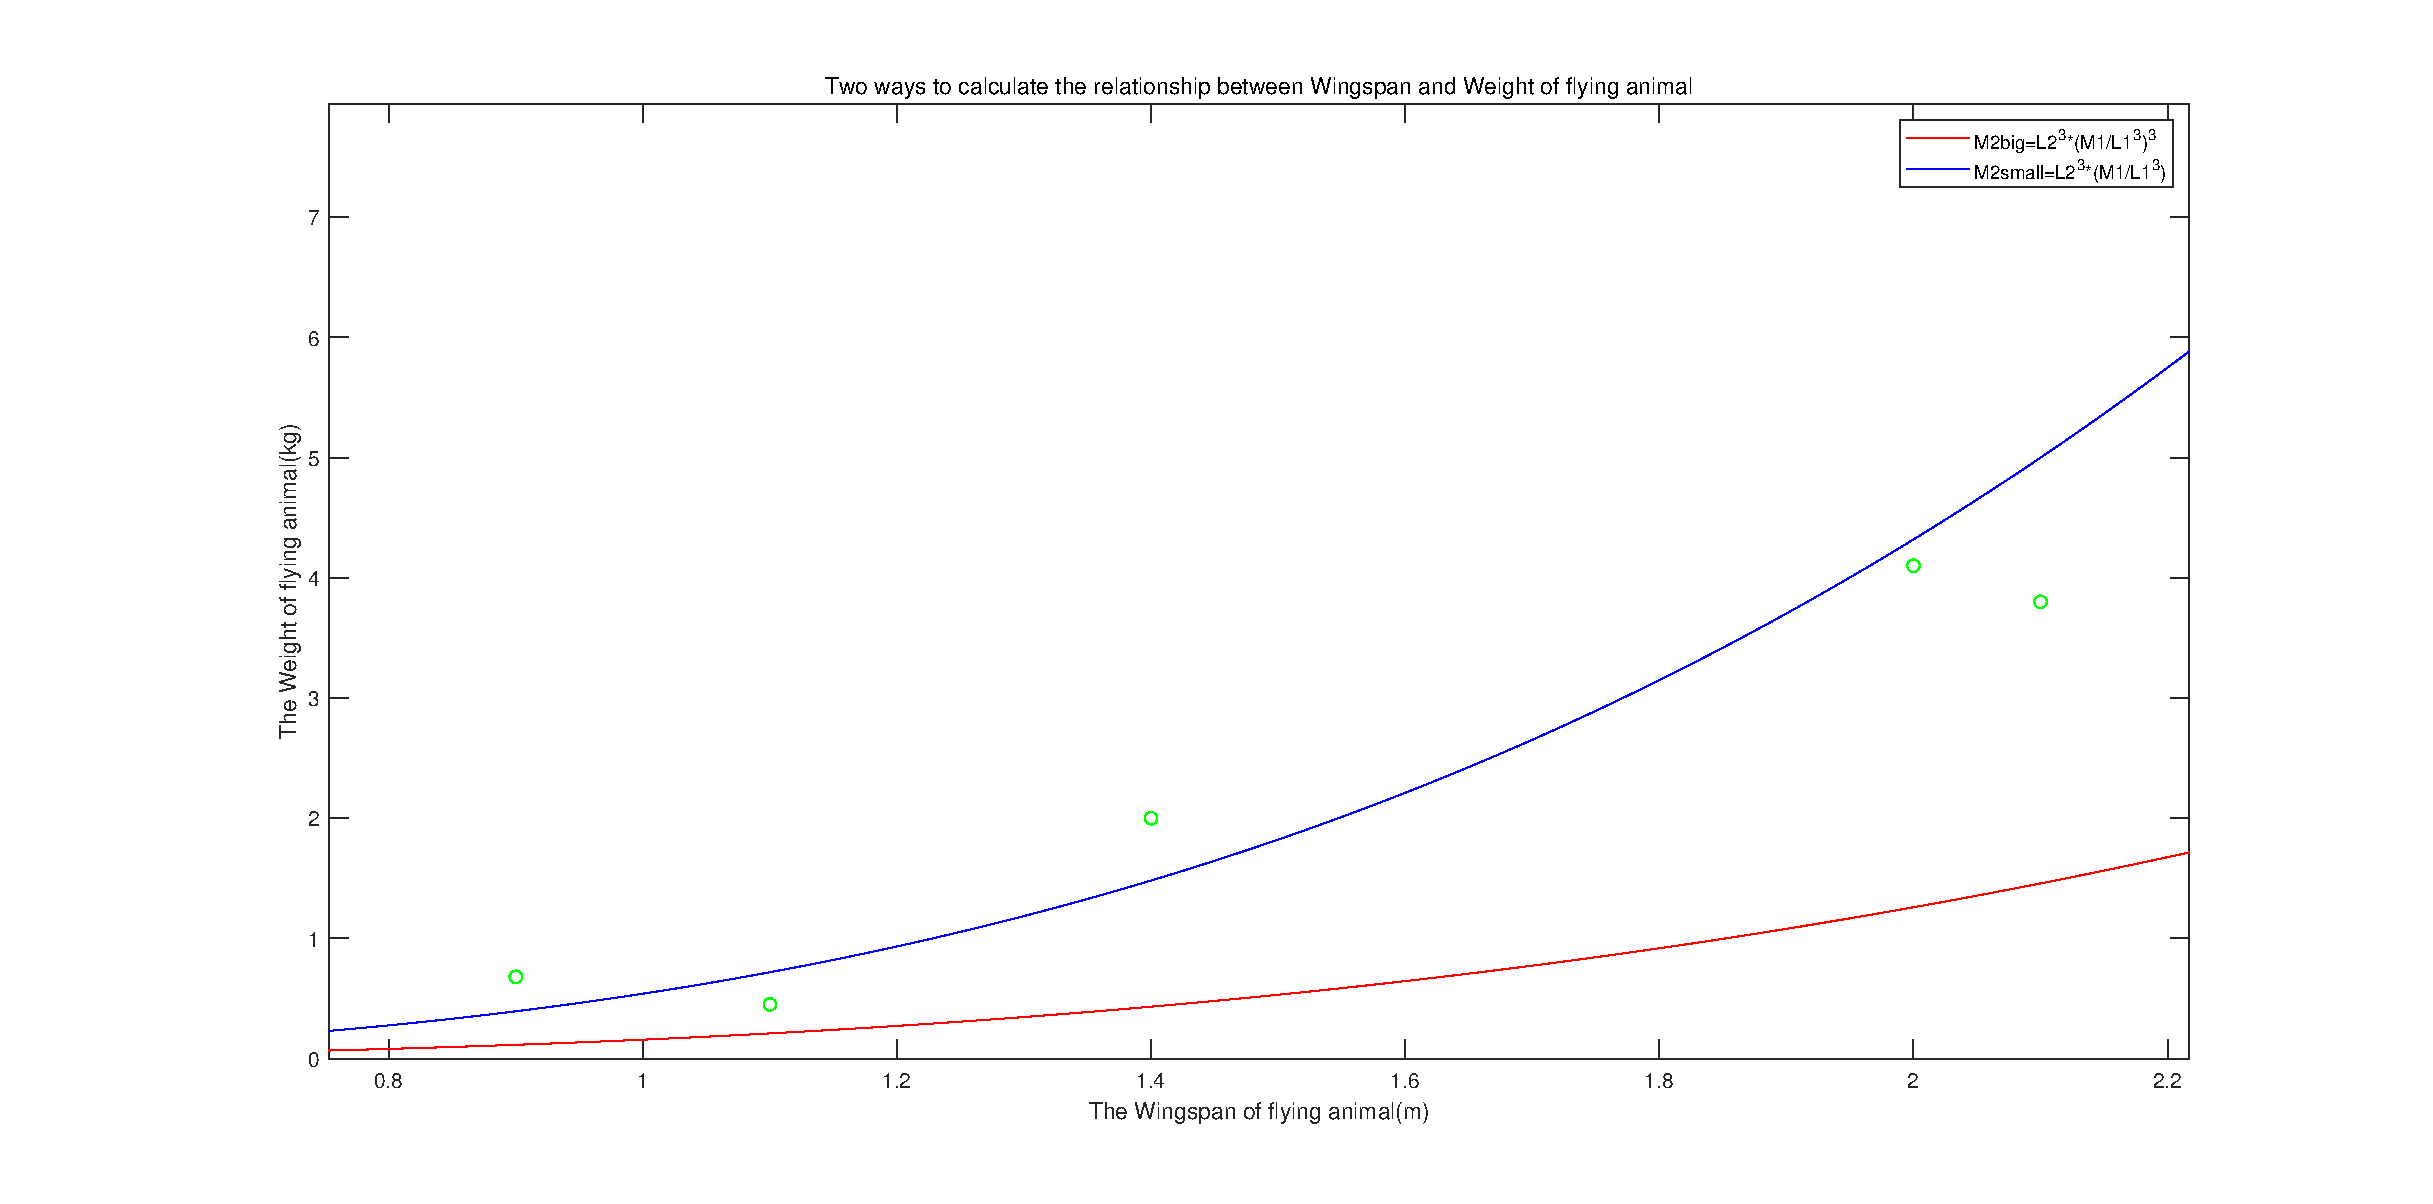
\includegraphics[width=14cm]{Two-ways-to-calculate-the-relationship-between-Wingspan-and-Weight-of-Dragon1.eps}}%小型动物拟合图
\begin{figure}[!htbp]
    \small  
	 \caption{Lower wingspan flighter fit equation(1)}\label{jj}
\end{figure}


		\centerline{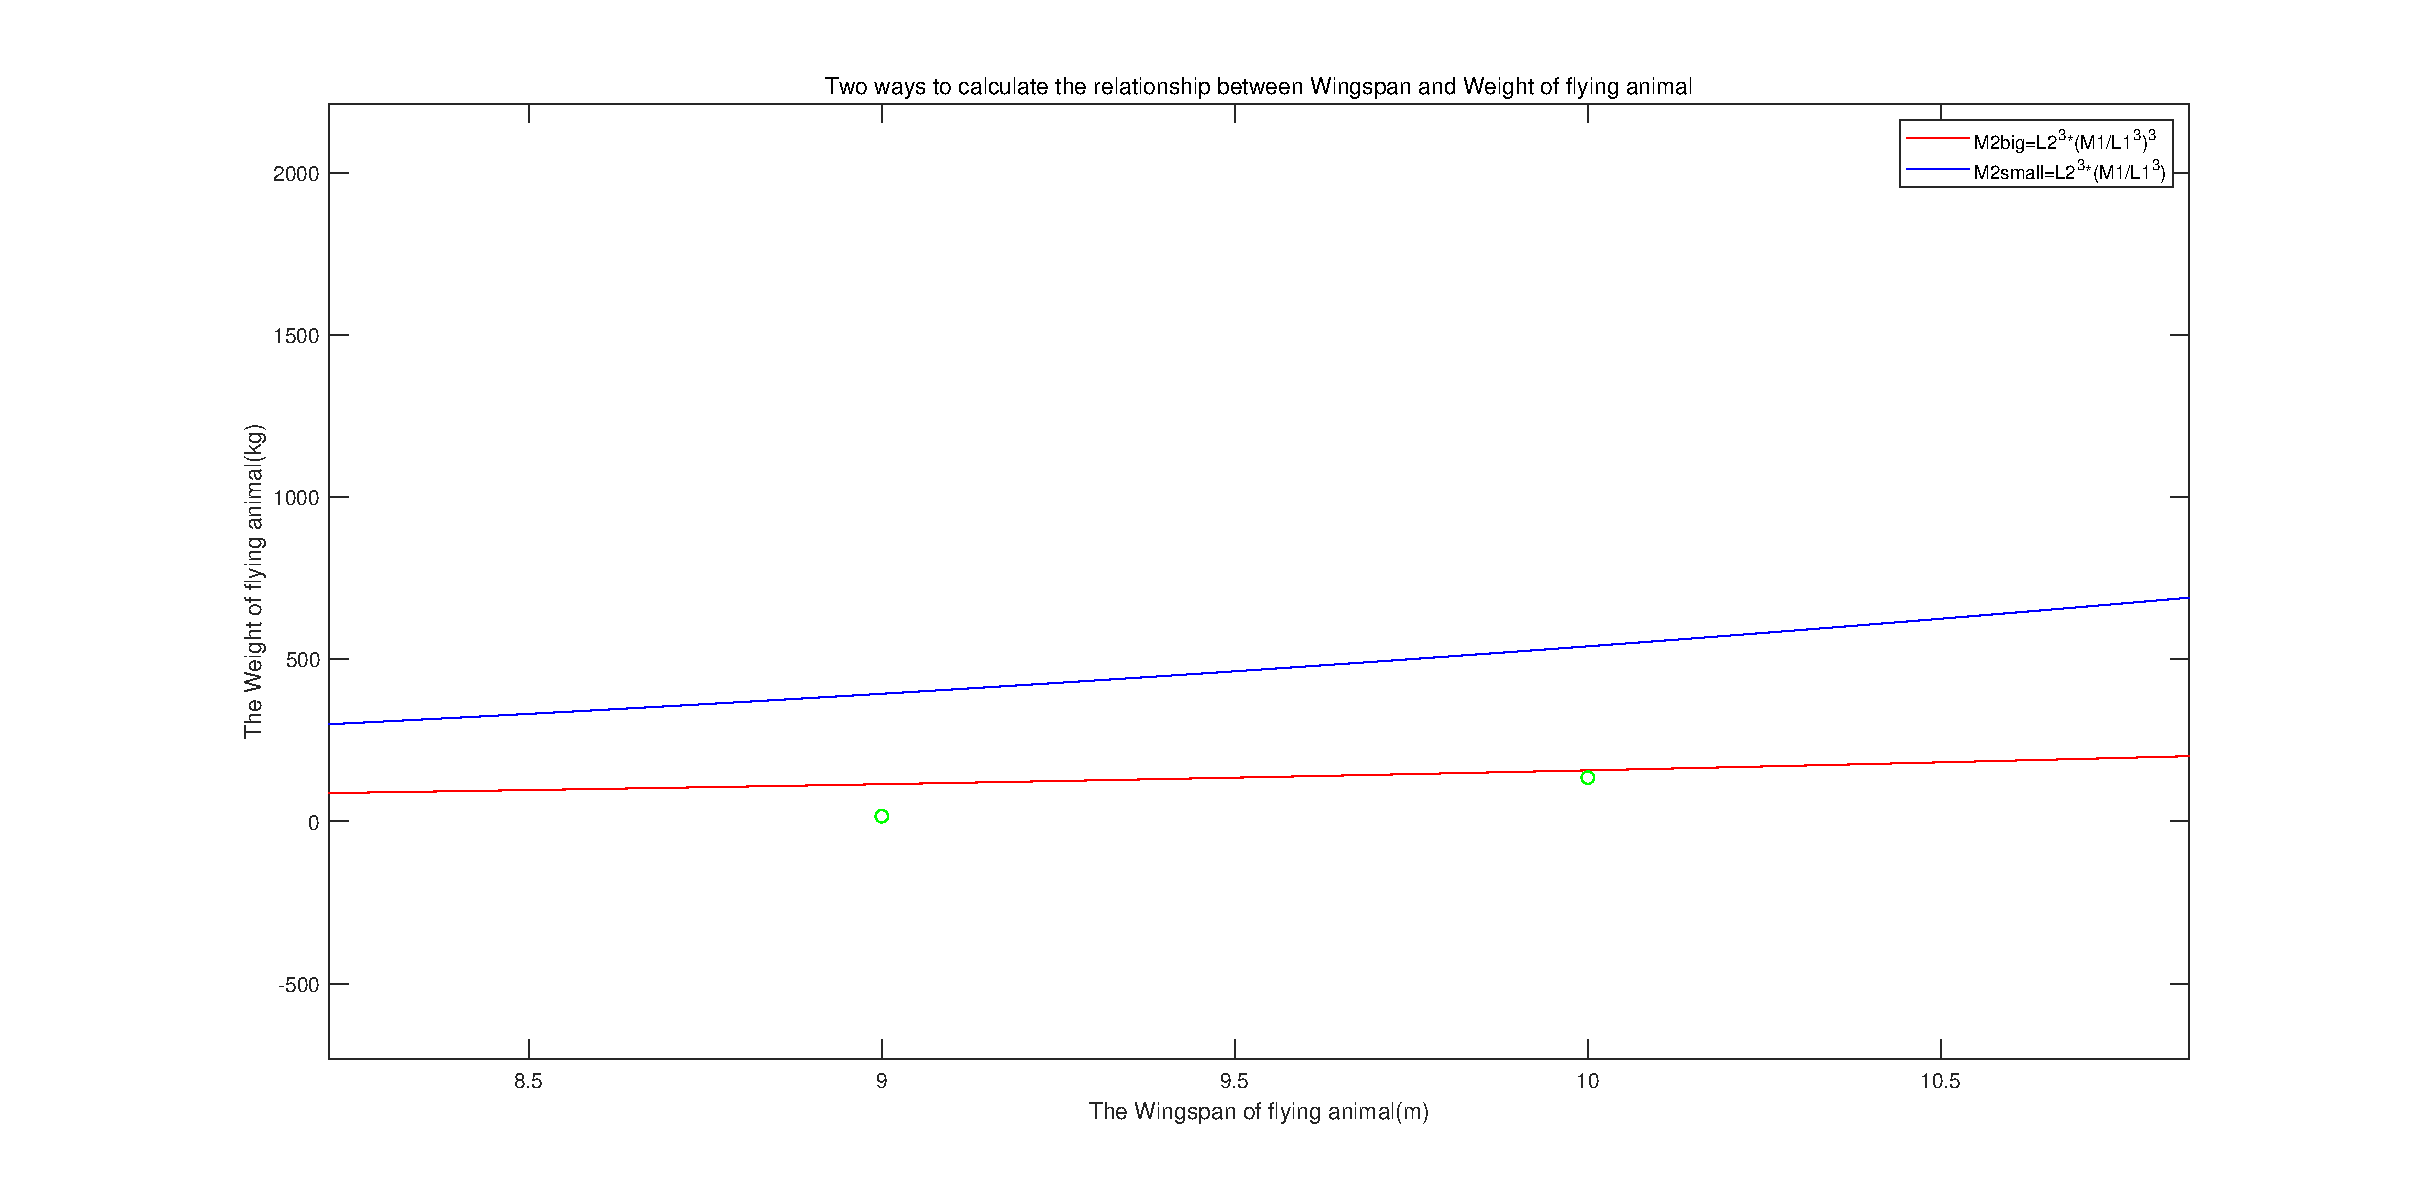
\includegraphics[width=14cm]{Two-ways-to-calculate-the-relationship-between-Wingspan-and-Weight-of-Dragon2.eps}}%大型动物拟合图
\begin{figure}[!htbp]
    \small
    \caption{Higher wingspan flighter fit equation(2)}\label{jj}
\end{figure}
We can conclude for small wingspan creature we use formula(1) to calculate its weight and for big wingspam's we use formula(2).


\subsubsection{Spray flame process}%喷火能量分析
From our assumption, we know the combustible is liquid. Then we think the Dragon as a flamethrower. Once a adult Dragon spray flame need about 14L liquid and about 12.155kg air. And as a result of contract, when full of the mixed gas, the volume of air cavity is 7mx2.5mx4m.\\
\begin{equation}
	Q_s=qV_0\frac{M_i}{M_0}.	%喷火能量
\end{equation}
Where:
\begin{itemize}
    \item $Q_s$ is the energy of spray flame(J);
    \item q is heat of combustion of biodiesel(3.3x10$^{14}$J/L);
    \item $V_0$ is the volume of air cavity(14L);
    \item $M_0$ is the weight of adult Dragon(66074.5kg);
    \item $M_i$ is the weight of growing Dragon(kg).
\end{itemize}
Dragon like eat roasted food and always spray flame for fun, so the energy using for spray flame should take a large proportion in its total energy consumption.

\subsubsection{Flying process}%%飞行过程分析

The P$_{aero}$(aerodynamic power) of bird flight process is divided into two part, one is P$_{ind}$(induced power), the other is P$_{pro}$(profile power).Induced power is the power required to maintain enough lift to overcome the force of gravity. Profile power is the power required to overcome body and wing resistance.

We simplified Dragon's flight to steady state flight$^{[4]}$,so the Dragon receives the same resistance and thrust, the same gravity and lift. 

So we can get induced power$^{[5]}$ of Dragon:
\begin{equation}
	P_{ind}=\frac{(mg)^2}{2VS_d\rho}.	%诱导功率
\end{equation}
Where
\begin{itemize}
    \item m is the weight of Dragon(kg);
    \item g is gravity(N/kg);
    \item V is the speed of Dragon(m/s);
    \item S$_d$ is the area size of Dragon wing(m$^2$);
    \item $\rho$ is the density of air(kg/m$^3$).
\end{itemize}

We also get profile power of Dragon:
\begin{equation}
	P_{pro}=\frac{\rho V^3S_dC_{Db}}{2}.	%外形功率
\end{equation}
Where
\begin{itemize}
    \item $C_{Db}$ is drag coefficient$^{[6]}$, value is 0.1;
\end{itemize}

Because there is pressure above and below the wings of Dragon. The air in the lower part of the wing will also move to the upper part of the wing. This air will form a nest in the upper part of the wing together with the air moving down the wing. That means pressure can offset portion of resistance, that's why birds save power when gliding. This pressure difference is proportional to S$_d$ and $\rho$. So we set up a correction factor$^{[5]}$:
\begin{equation}
	P_{pro}^{'}=\alpha P_{pro}.	%修正后的外形功率
\end{equation}
Where
\begin{itemize}
    \item $P_{pro}^{'}$ is corrected profile power(W);
	 \item $\alpha$ is a correction coefficient to account for the difference between the size of the wing disc and the actual tube of air displaced by the bird's wings. We set its value to 0.02
\end{itemize}

Using equations(3) and (5) we can easily derive equation(6):
\begin{equation}
	W_f=P_{aero}=P_{ind} + P_{pro}^{'}.	%总功率
\end{equation}


\centerline{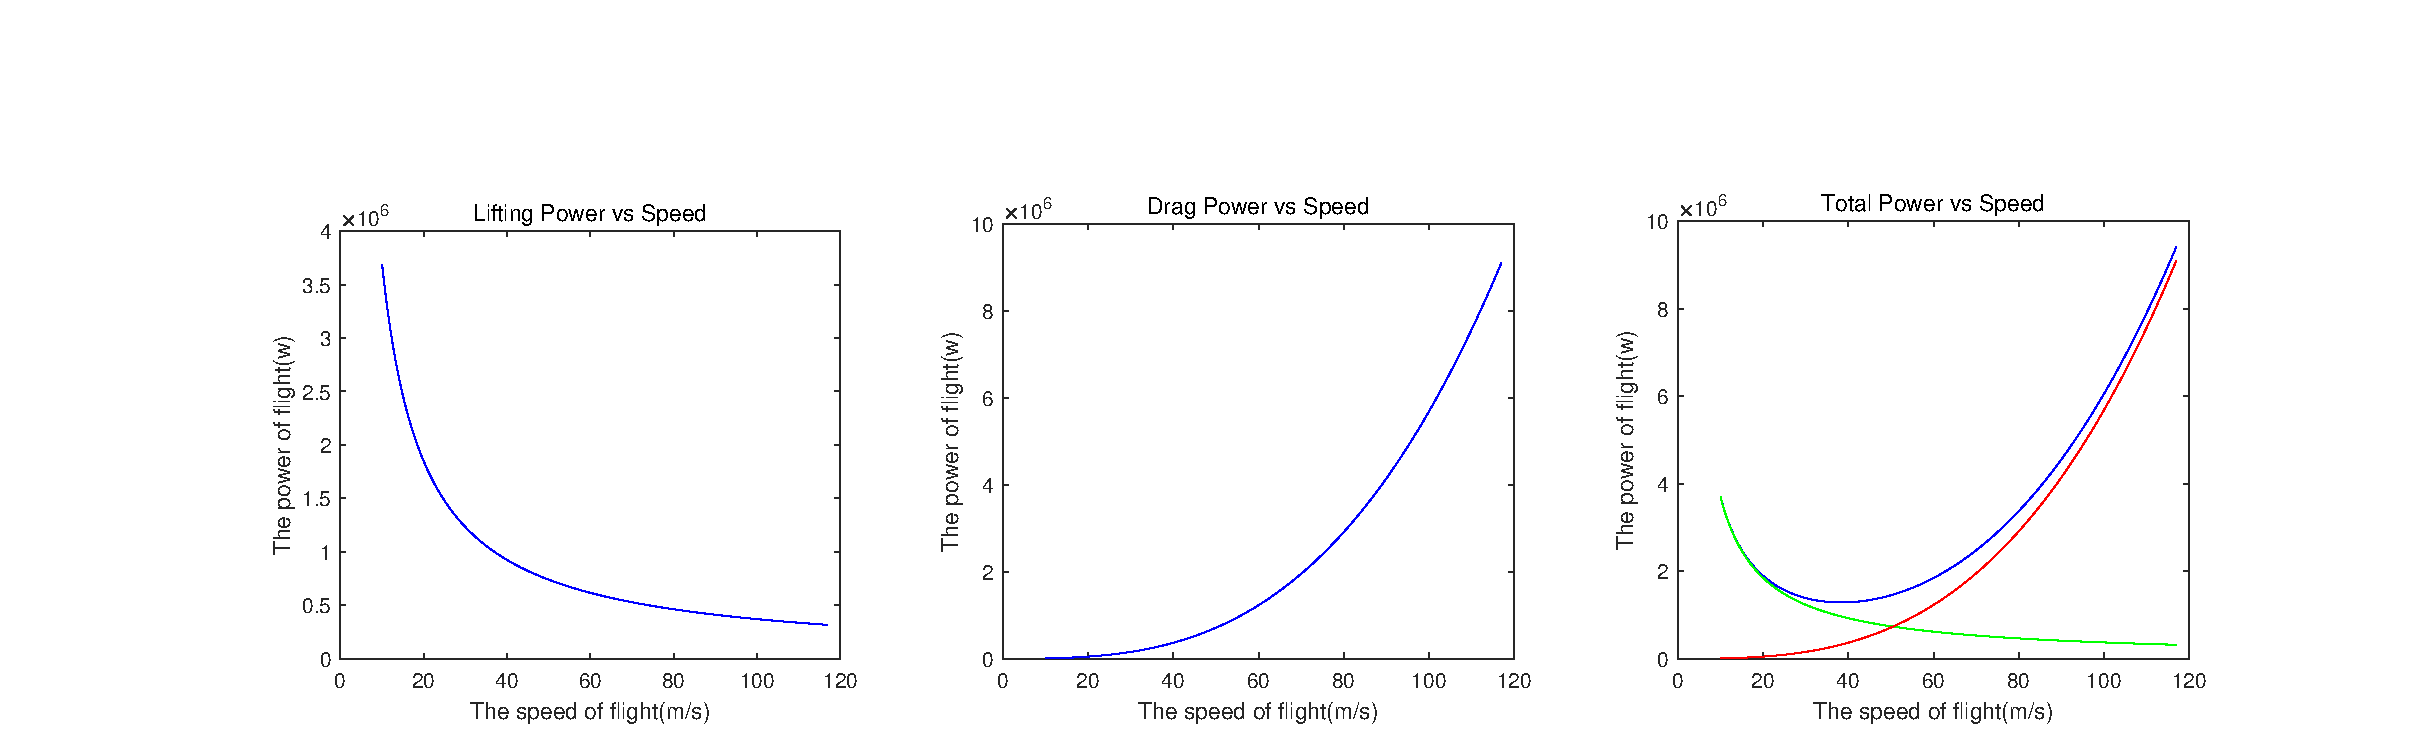
\includegraphics[width=20cm]{The-relationship-between-speed-and-power-of-flying0.eps}}%速度与功率关系图
\begin{figure}[!htbp]
    \small
    \caption{The relationship between speed and power of flying}\label{jj}
\end{figure}
The left figure shows the power required to increase the power.The middle figure shows the power lift required to overcome the resistance.The right figure shows The power required to increase the power and lift required to overcome the resistance provides the total power required for flight.


\subsubsection{Activity range model}%%活动范围模型
Dragon is a vivacious creature. So we propose these factors:
\begin{itemize}
    \item The Dragon total activity nine hours in three days;
	 \item The Dragon can only change direction to forward or right or left;
	 \item The Dragon change direction at most once per six seconds.
\end{itemize}
Then we draw this picture to show the furthest activity range:

\centerline{\includegraphics[width=14cm]{random_walk.png}}%游走模拟图
\begin{figure}[!htbp]
    \small
    \caption{The point shows the furthest place where the Dragon can travel base on these factors}\label{jj}
\end{figure}
From the novel, we know the highest speed of Dragon is 400km/h. So, we hypothesis the speed of Dragon is 200km/h. According to the figure above, we can calculate: each pixel is $\frac{1}{3}km$. The coordinate of the furthest point is(-571,-982). We conclude the radius of activity range of Dragon is 378.6 km; the area of activity range of Dragon is 450 thousand km$^2$


\subsubsection{Diet structure of Dragon}%%龙的饮食结构
In order to understand diet structure of Dragon. Analogy the diet structure of golden eagle$^{[1]}$, we speculate Dragon's diet structure:\\

\centerline{\includegraphics[width=14cm]{pie-iceland.pdf}}%冰岛食物结构饼状图
\begin{figure}[!htbp]
    \small
    \caption{Food structure of Dragon in Iceland}\label{jj}
\end{figure}


\centerline{\includegraphics[width=14cm]{pie-ireland.pdf}}%爱尔兰食物结构饼状图
\begin{figure}[!htbp]
    \small
    \caption{Food structure of Dragon in Ireland}\label{jj}
\end{figure}

\centerline{\includegraphics[width=14cm]{pie-morocco.pdf}}%摩洛哥食物结构饼状图
\begin{figure}[!htbp]
    \small
    \caption{Food structure of Dragon in Morocco}\label{jj}
\end{figure}

\subsubsection{Relationship between metabolism and ambient temperature}%%代谢与环境温度关系
The surface area of the Dragon is:
\begin{equation}
	S_w=\pi \left(\frac{b}{2}\right)^2.	%龙翼表面积
\end{equation}	
Where: 
\begin{itemize}
    \item $S_w$ is the surface area of Dragon wingspan(m$^2$);
	 \item b is the length of Dragon wingspan(m).
\end{itemize}
We analogy the body of Dragon as cylinder.So the surface area of the Dragon is:
\begin{equation}
	A=2\pi r + 2\pi rl + 4\alpha S_w.	%龙的表面积
\end{equation}	
Where:
\begin{itemize}
    \item $A$ is the surface area of Dragon($m^2$);
	 \item $b$ is the section radius of Dragon(m);
	 \item $l$ is the length of Dragon(m);
	 \item $\alpha$ is the correction factor which value is 0.1. 
\end{itemize}
A typical metabolic heat production is as follow:
\begin{equation}
	Q = C A \left[\left(\frac{T_1}{100}\right)^4 - \left(\frac{T_2}{100}\right)^4 \right].	%普遍散热
\end{equation}	
\begin{itemize}
    \item $Q$ is metabolic heat production($K_{cal}/h$);
	 \item $C$ is total emissivity of object;
	 \item $T_1$ is the temperature of object(K);
	 \item $T_2$ is the ambient temperature(K).
\end{itemize}
And metabolic heat production of human$^{[8]}$ is as follow:
\begin{equation}
	h_r=\varepsilon_s \sigma k.	%人体散热
\end{equation}	
\begin{equation}
	Q = h_r A \left[\left(\frac{T_1}{100}\right)^4 - \left(\frac{T_2}{100}\right)^4 \right].	%人体散热
\end{equation}	
Where: 
\begin{itemize}
	 \item $\varepsilon$ is emissivity of the human surface;
	 \item $\sigma$ is Stefan-Boltzmann Constant, $K_{cal}/m^2 h ^{\circ}k^4$;
	 \item $k$ is temperature factor of radiation heat exchange = $[(T_s+273)^2+(T_i+273)^2]*[(T_s+273)+(T_i+273)], ^{\circ}k^3$;
	 \item $h_r$ is radiative heat transfer coefficient derived by using the absorption factor method, $K_{cal}/m^2h ^{\circ}C$.
\end{itemize}
Metabolic equation of dragon is as follow:
\begin{equation}
	\alpha = e^{\left(\frac{T_1-T_2}{T_2-T_3}\right)\cdot\left(\frac{A}{B}\right)}
\end{equation}
\begin{equation}
	E_s=\alpha \cdot 4.1W^{0.751}.	%代谢公式的修正因子
\end{equation}
Where:
\begin{itemize}
	 \item $\alpha$ is correction factor for metabolic equation;
	 \item $T_1$ is body temperature of Dragon(K);
	 \item $T_2$ is body temperature of human(K);
	 \item $T_3$ is body temperature of warm-blooded animal(K);
	 \item $A$ is food intake of warm-blooded animal, value is 10.7;
	 \item $B$ is food intake of cold-blooded animal, value is 0.78;
\end{itemize}
\centerline{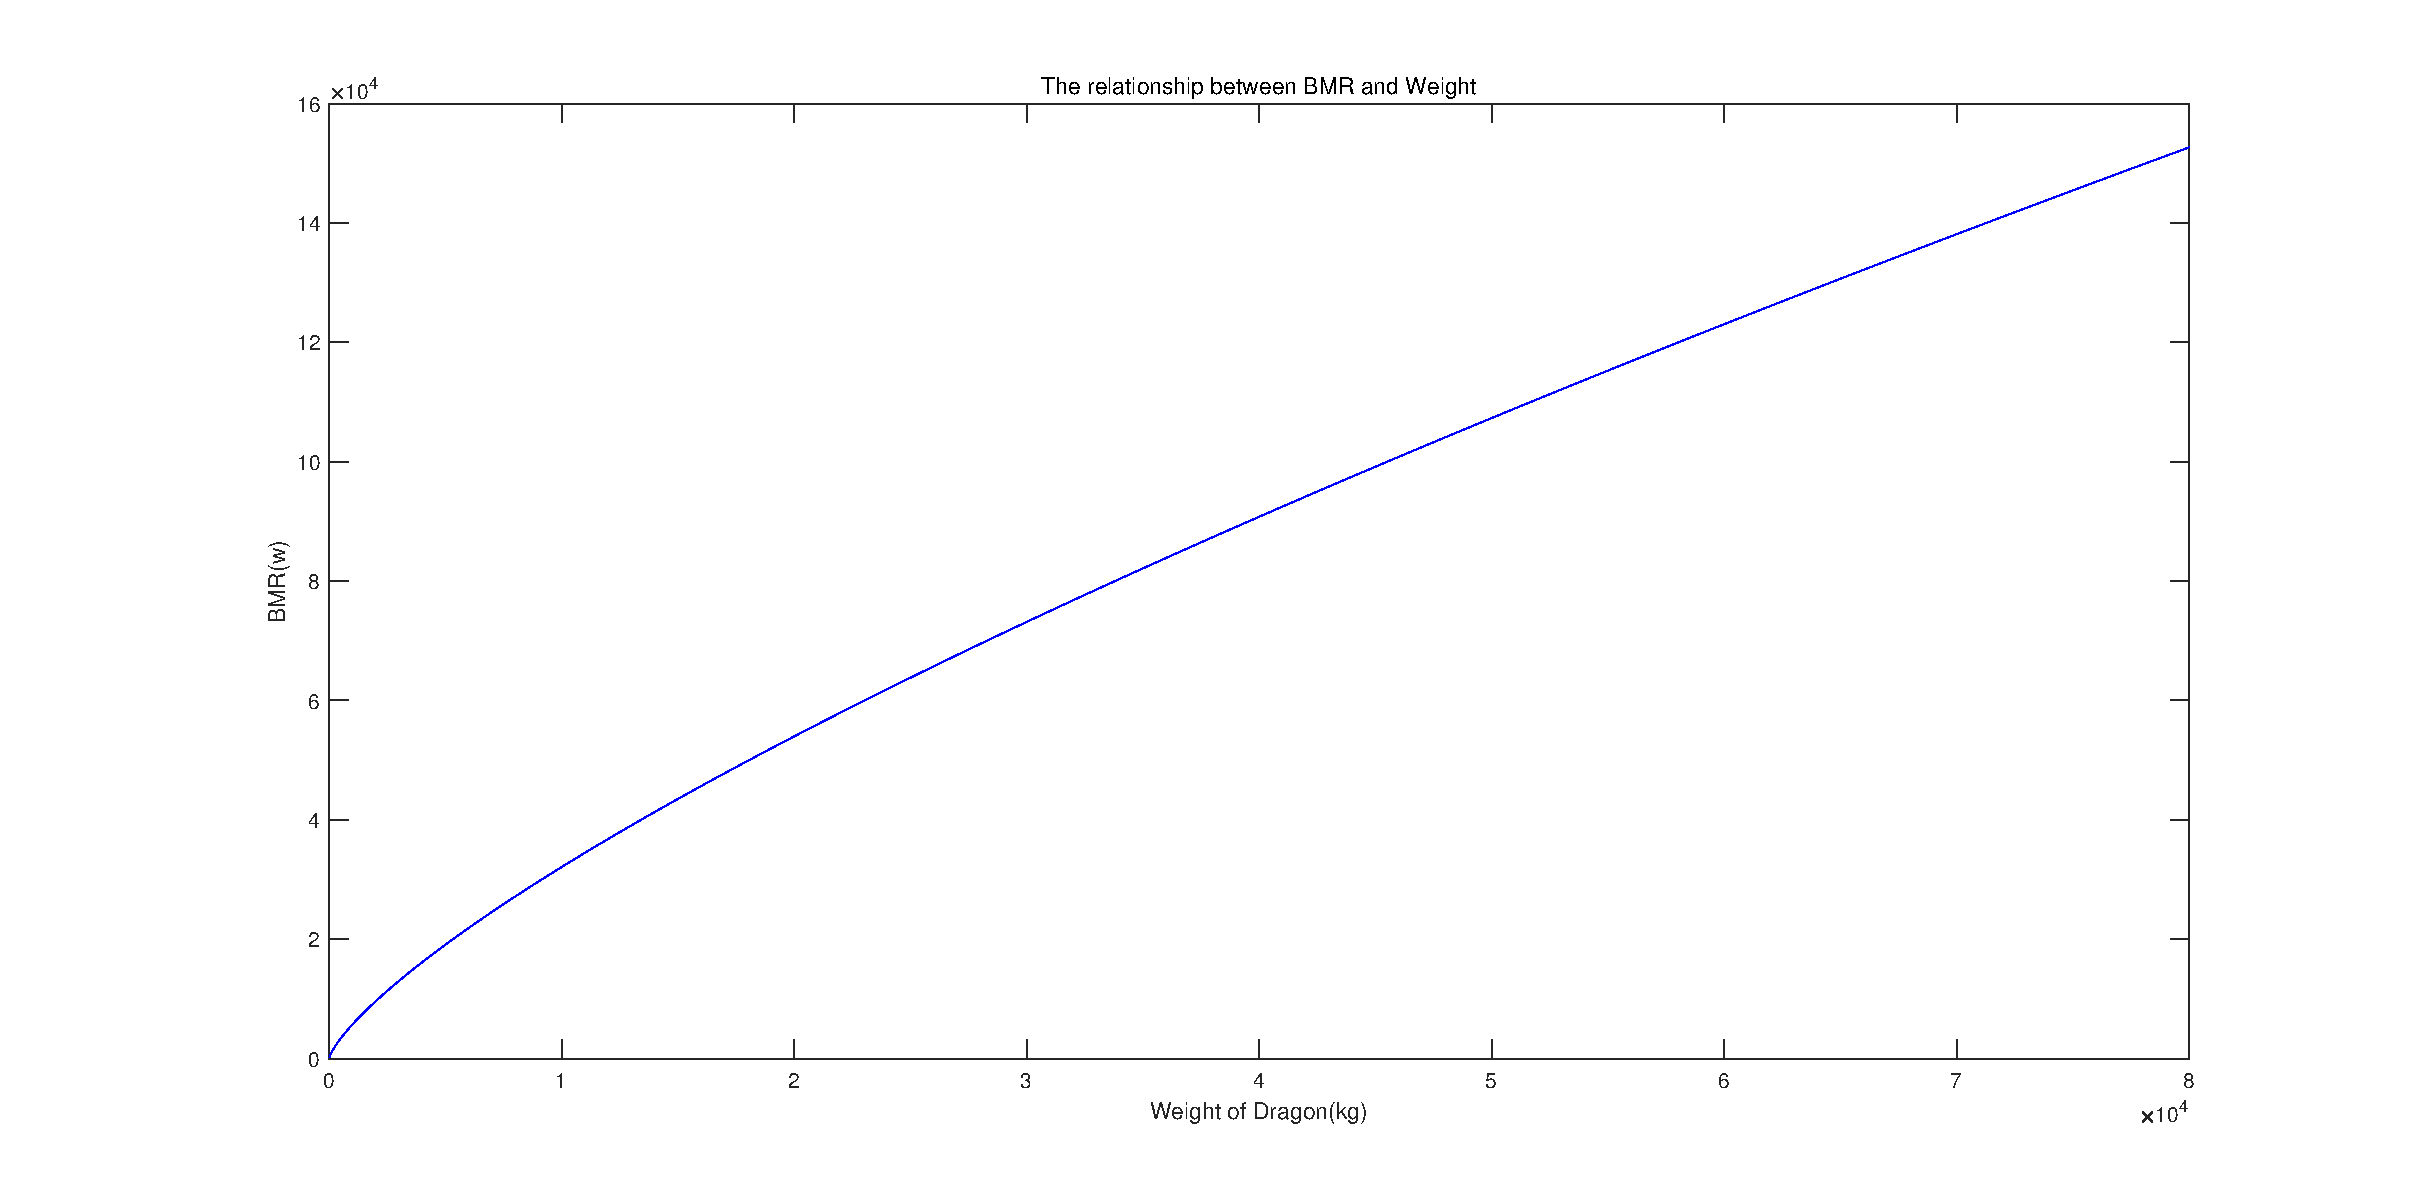
\includegraphics[width=20cm]{The-relationship-between-BMR-and-Weight.eps}}%BMR与龙体重关系
\begin{figure}[!htbp]
    \small
    \caption{Relationship between ambient temperature and metabolic heat production of Dragon}\label{jj}
\end{figure}
We calculate the dragon based on our corrected equation and test three data($T_1,T_2,T_3$):

\centerline{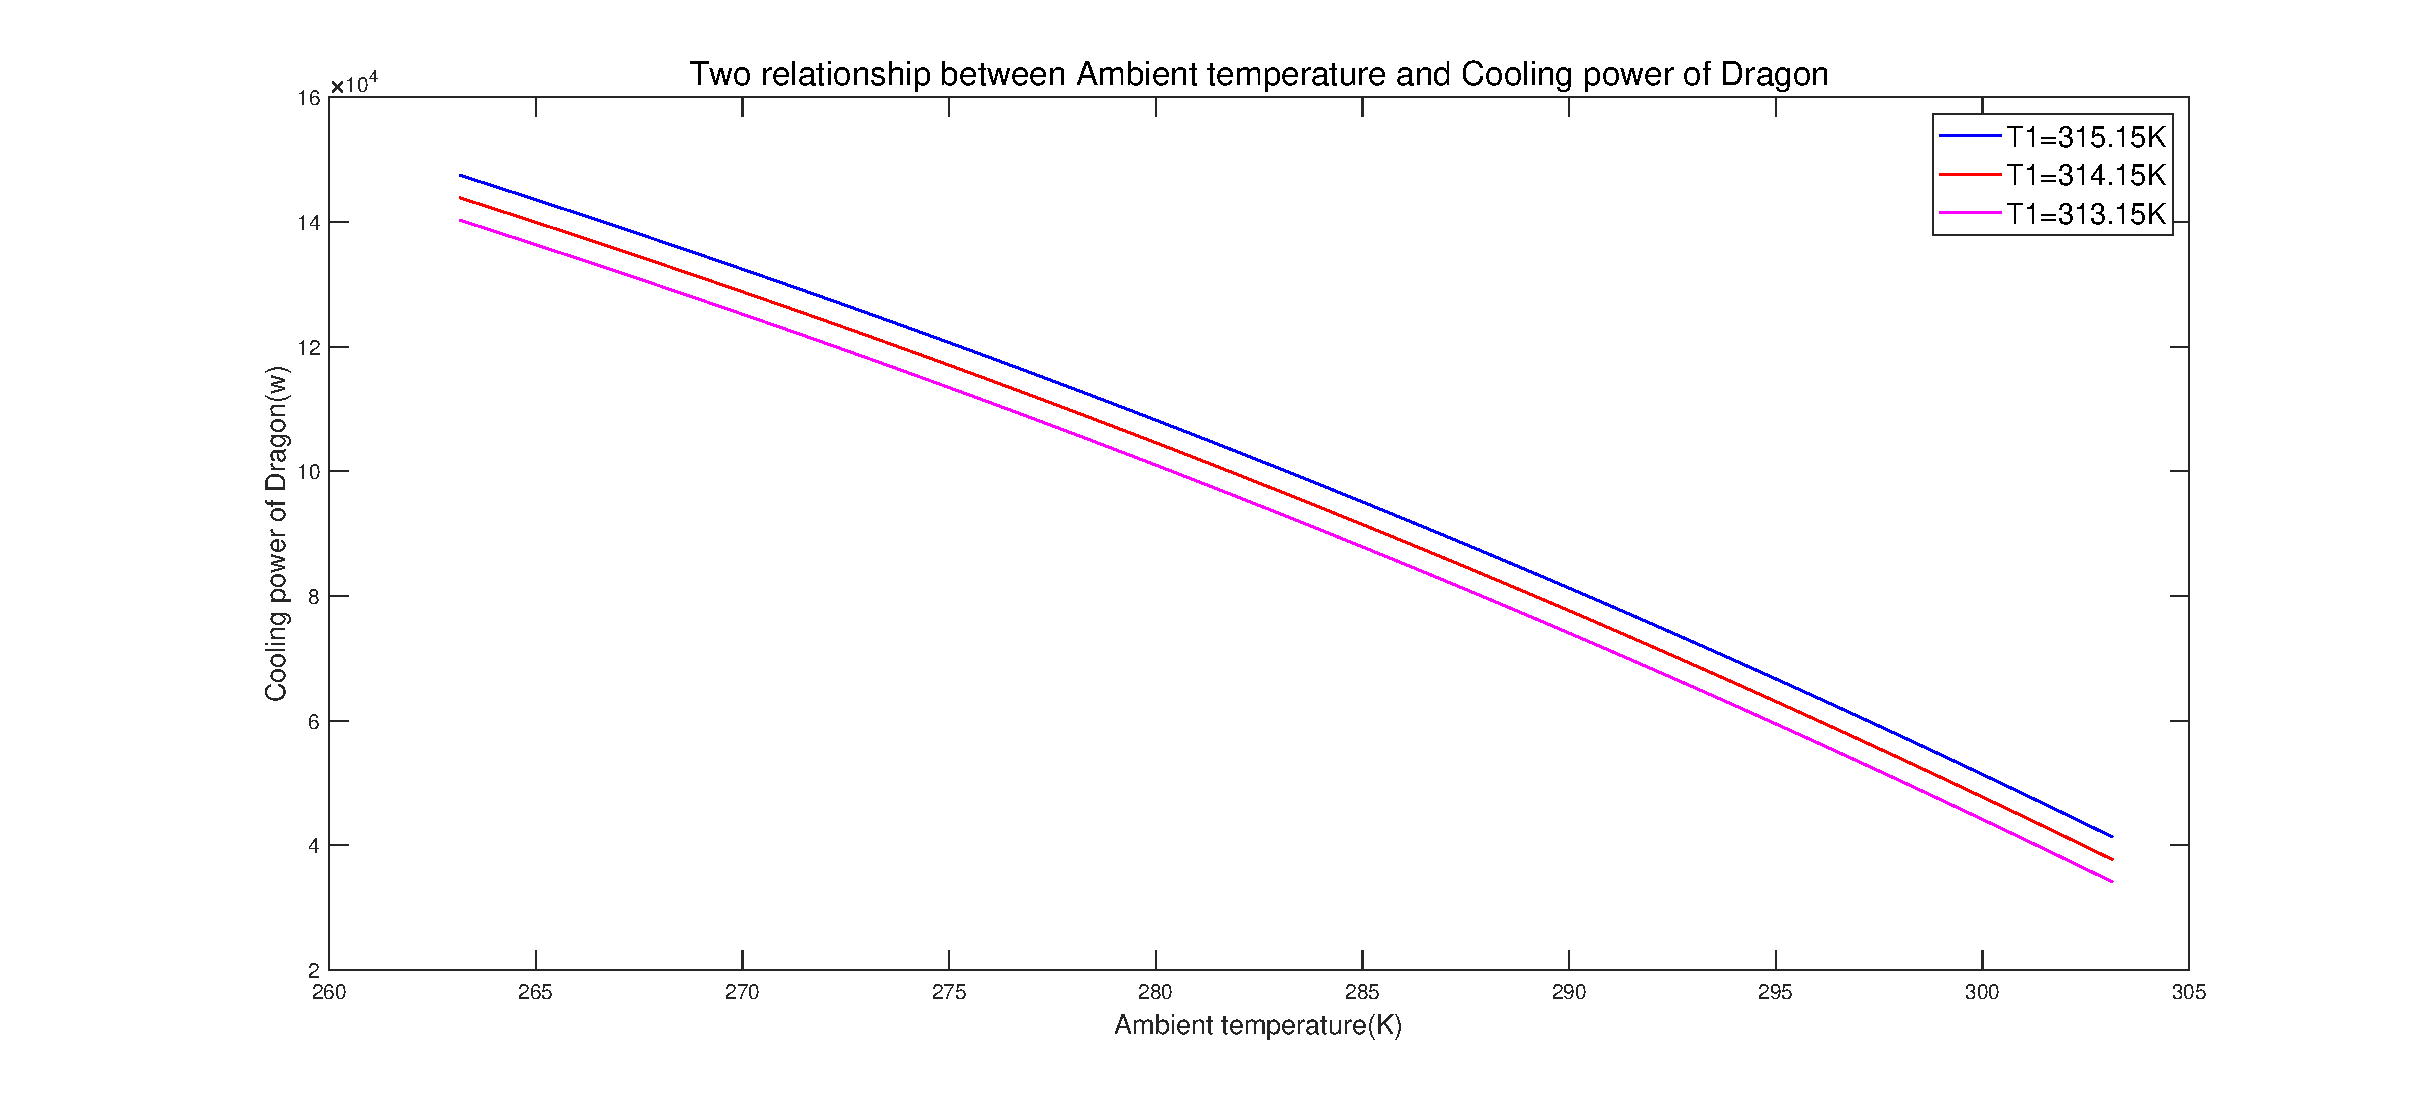
\includegraphics[width=20cm]{Two-relationship-between-Environment-temperature-and-Cooling-power-of-Dragon.eps}}%环境温度与龙体温关系
\begin{figure}[!htbp]
    \small
    \caption{Relationship between Environment temperature and Cooling power of Dragon}\label{jj}
\end{figure}

\subsubsection{Dragon growth model}%模型
Warm-blooded animal only turn 2\% of energy into a part of its body.They use 77\% of intake energy to keep alive.The extra part is not used and excreted as stool,we can know only 2\% of energy is used for growth$^[7]$.
Based above, we consider that Dragon assimilation efficient, so we correct 77\% to 78\%.\\
In line with the drama, child Dragon we use artificial breeding. Generally, the meat assimilation rate is between 80 and 90 percent. The dragon is the top of the food chain, and we set it to 90 percent. (The assimilation rate can be set to a physical quantity here)
We assume child Dragon is feeded with beef and mutton.
\begin{equation}
	90\%W_{in}-W_f-W_d-W_s=W_{g} .	%
\end{equation}
\begin{equation}
	M_i=\left[0.09M_1-0.002M_1-0.0984M_1^{\frac{3}{4}}-5.4*10^{-4}M_1^{\frac{13}{12}}-3.9*10^{-4}*M_1^{\frac{17}{12}}\right]*0.34+M_0 .	%
\end{equation}
Where:
\begin{itemize}
	 \item $W_f$ is energy used for flight;
	 \item $W_d$ is energy used for metabolic;
	 \item $W_s$ is energy used for spray flame;
	 \item $W_{in}$ is energy from food intake;	 
	 \item $W_g$ is energy used for grow;
\end{itemize}

According equation(1) and equation(2), we found the model of adult Dragon and child Dragon is different:

\centerline{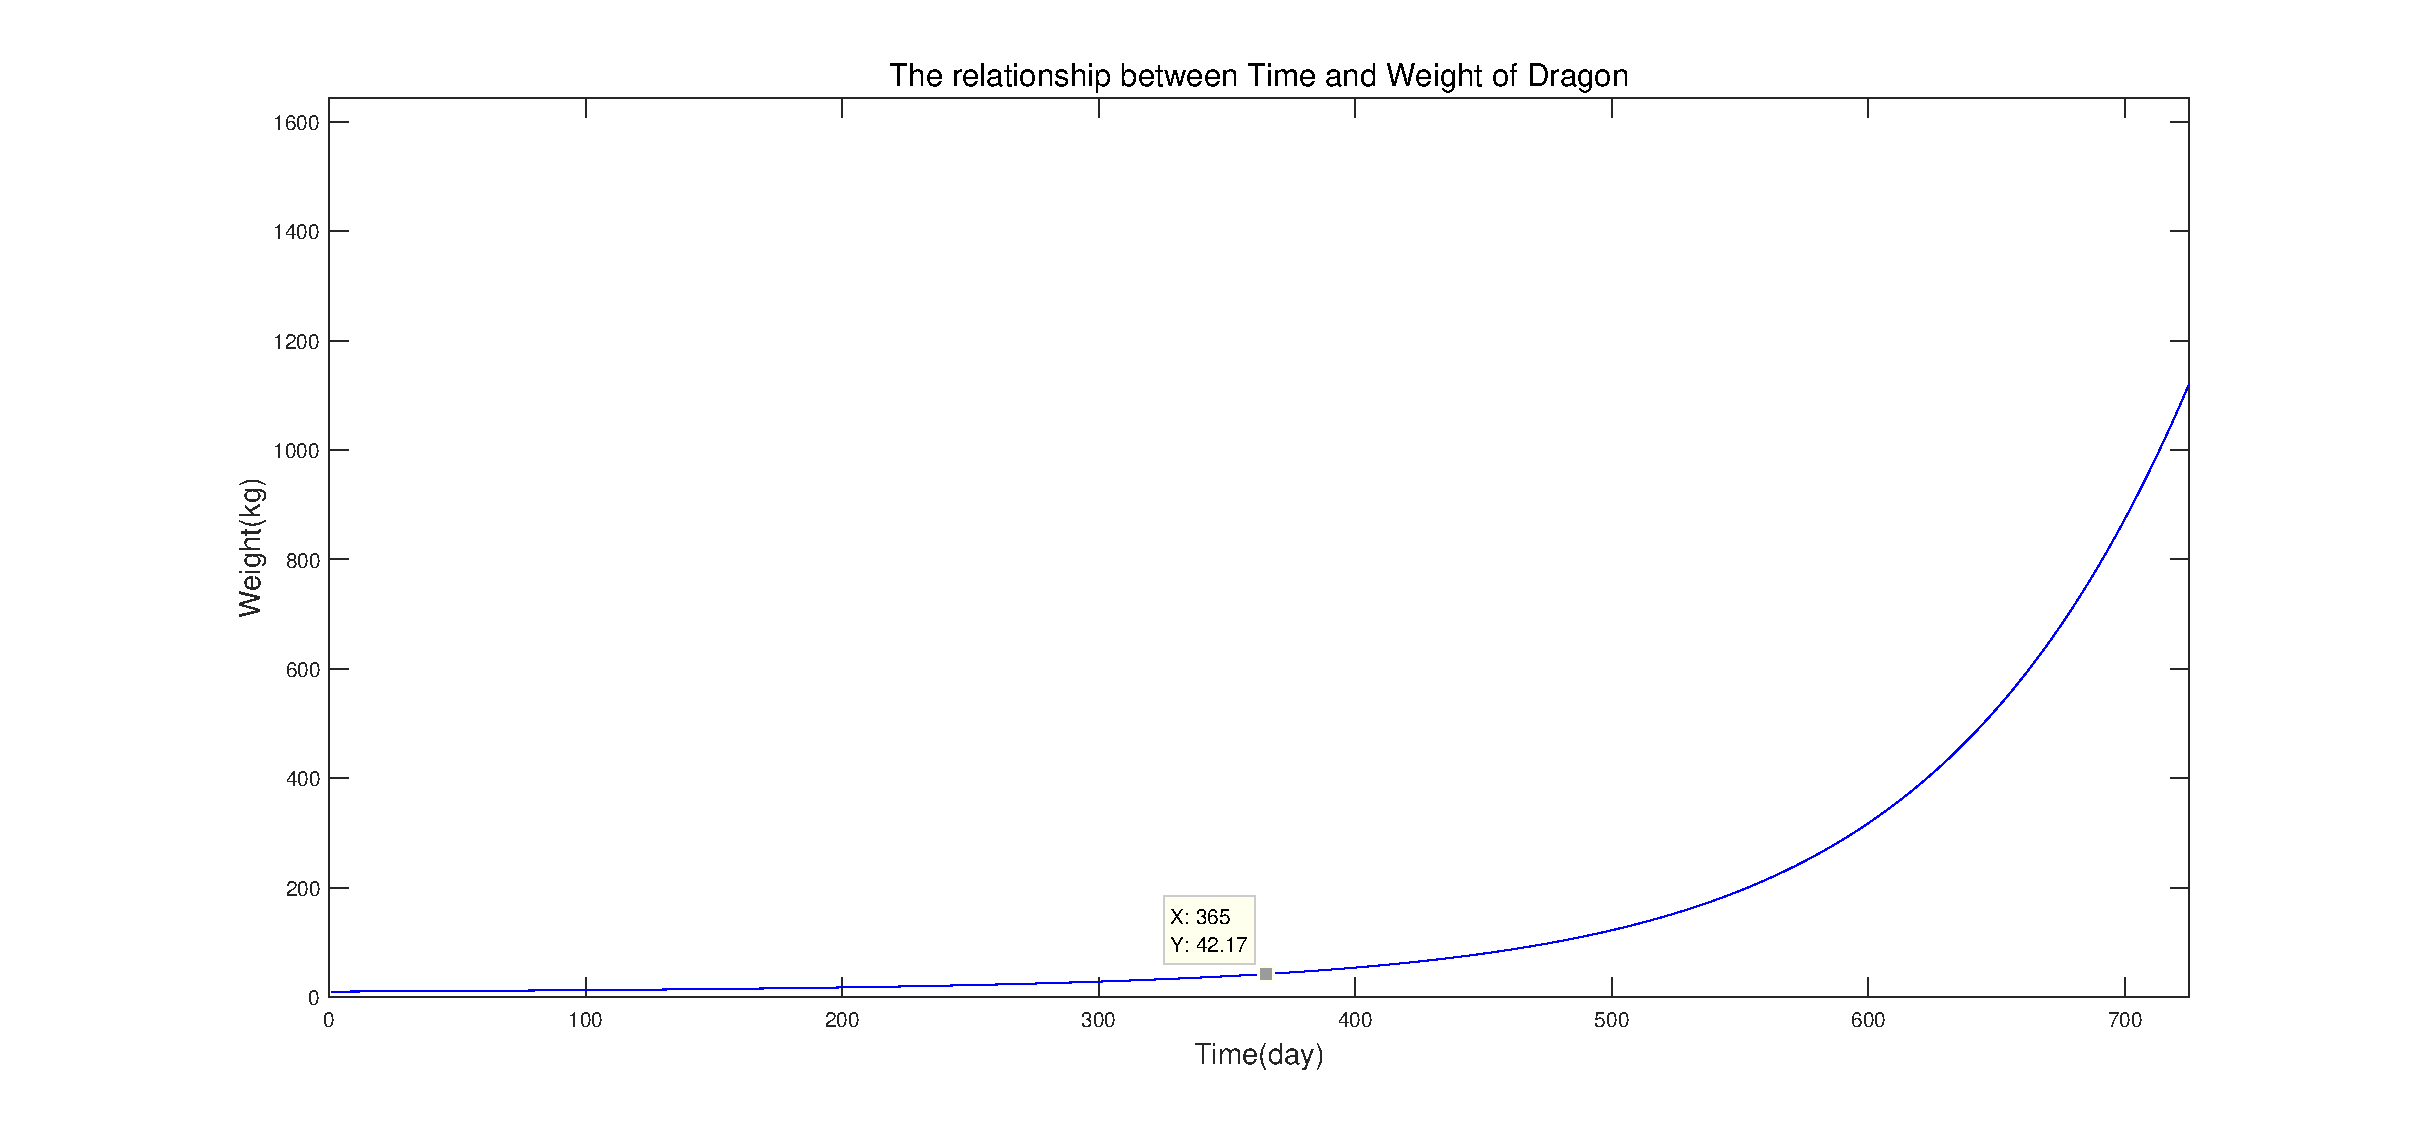
\includegraphics[width=20cm]{grow2.eps}}%社区与三龙的体重
\begin{figure}[!htbp]
    \small
    \caption{The relationship between time and weight of Dragon}\label{jj}
\end{figure}

In conclusion, in this model, child Dragon weight gain is quadratic with time, and when the time is one year, the dragon’s weight is about 40 kg.
t is consistent with the growth of the dragon after one year. Explain that the curve of the child dragon is still accurate. And this curve shows that the dragon has increased significantly over time, and the second half of the curve is significantly faster than the first half, so that over time,
The weight gain rate is getting bigger and bigger, and more and more energy is needed.


\subsection{Energy flow between Dragon and ecology Model}%能量模型
Assumption: Utilization rate is 100 percent. All energy is produce to the Dragon and don't consider ecological recovery rate.The higher temperature is, the faster Dragon assimilation is. So warmer area is more easy for Dragon to get emnergy, warmer area is better for Dragon growth. Meanwhile, considered ecosystem's utilization of solar energy, warm area is better than extremely cold or hot area.So we think artic is the least one, arid is more ,warm is the most.
\subsubsection{Relationship between weight of Dragon and climate}%计算生存所需面积
To simplify the model we set efficiency of assimilation to 90 percent, and set rate of growth to 2 percent.
\begin{equation}
	W_f+W_d+W_s=88\%W_{in} .	%摄入能量
\end{equation}

In order to analysis nutritional structure of Dragon and to find out how energy flows in the ecosystem, we draw the following figure:

\centerline{\includegraphics[width=14cm]{food-chain.pdf}} %食物链
\begin{figure}[!htbp]
    \small
    \caption{Simplified food chain of Dragon}\label{jj}
\end{figure}
\begin{equation}
	\frac{90\%W_{in}}{x}=20\% .	%
\end{equation}
\begin{equation}
	\frac{x}{y}=10\% .	%
\end{equation}
\begin{equation}
	\frac{y}{z}=1\% .	%
\end{equation}
Where:
\begin{itemize}
	 \item $x$ is assimilation amount of sheep or cattle;
	 \item $y$ is quantity of grass;
	 \item $z$ is Daily average radiant energy of light;
\end{itemize}
These three country have various climate(Morocco is tropical desert climate, Ireland is temperate maritime climate,Iceland is Tundra climate), so different daily average radiant energy of light and grassland coverage effect our model a lot:
\begin{equation}
	S=\frac{z}{\gamma\beta}	%面积
\end{equation}
Where:
\begin{itemize}
	 \item S is area(m$^2$);
	 \item $\gamma$ is Daily average radiant energy of light;
	 \item $\beta$ is grassland coverage;
\end{itemize}
\begin{table}[!htbp]
\begin{center}
\caption{The different $\gamma$ and $\beta$ in various area}
\begin{tabular}{lccc}
    \toprule
    Country& Ireland& Iceland& Morocco\\
    \midrule
    $\gamma_i$& 3.1469& 2.2457& 5.9101\\
    $\beta_i$& 0.06& 0.02& 0.0126\\
    \bottomrule
\end{tabular}\label{h}
\end{center}
\end{table}
\centerline{\includegraphics[width=20cm]{111.eps}}
\begin{figure}[!htbp]
    \small
    \caption{relationship of weight and area}\label{jj}
\end{figure}
As shown in the figure, undering different climate, relationship of weight of Dragon and required area. At the same area,various climate cause different upper limit of weight of Dragon. artic is the least one, arid is more ,warm is the most. So in the same area, climate will effect weight of Dragon. Therefore, commend to raise Dragon in warm area to get more weight. \\

\centerline{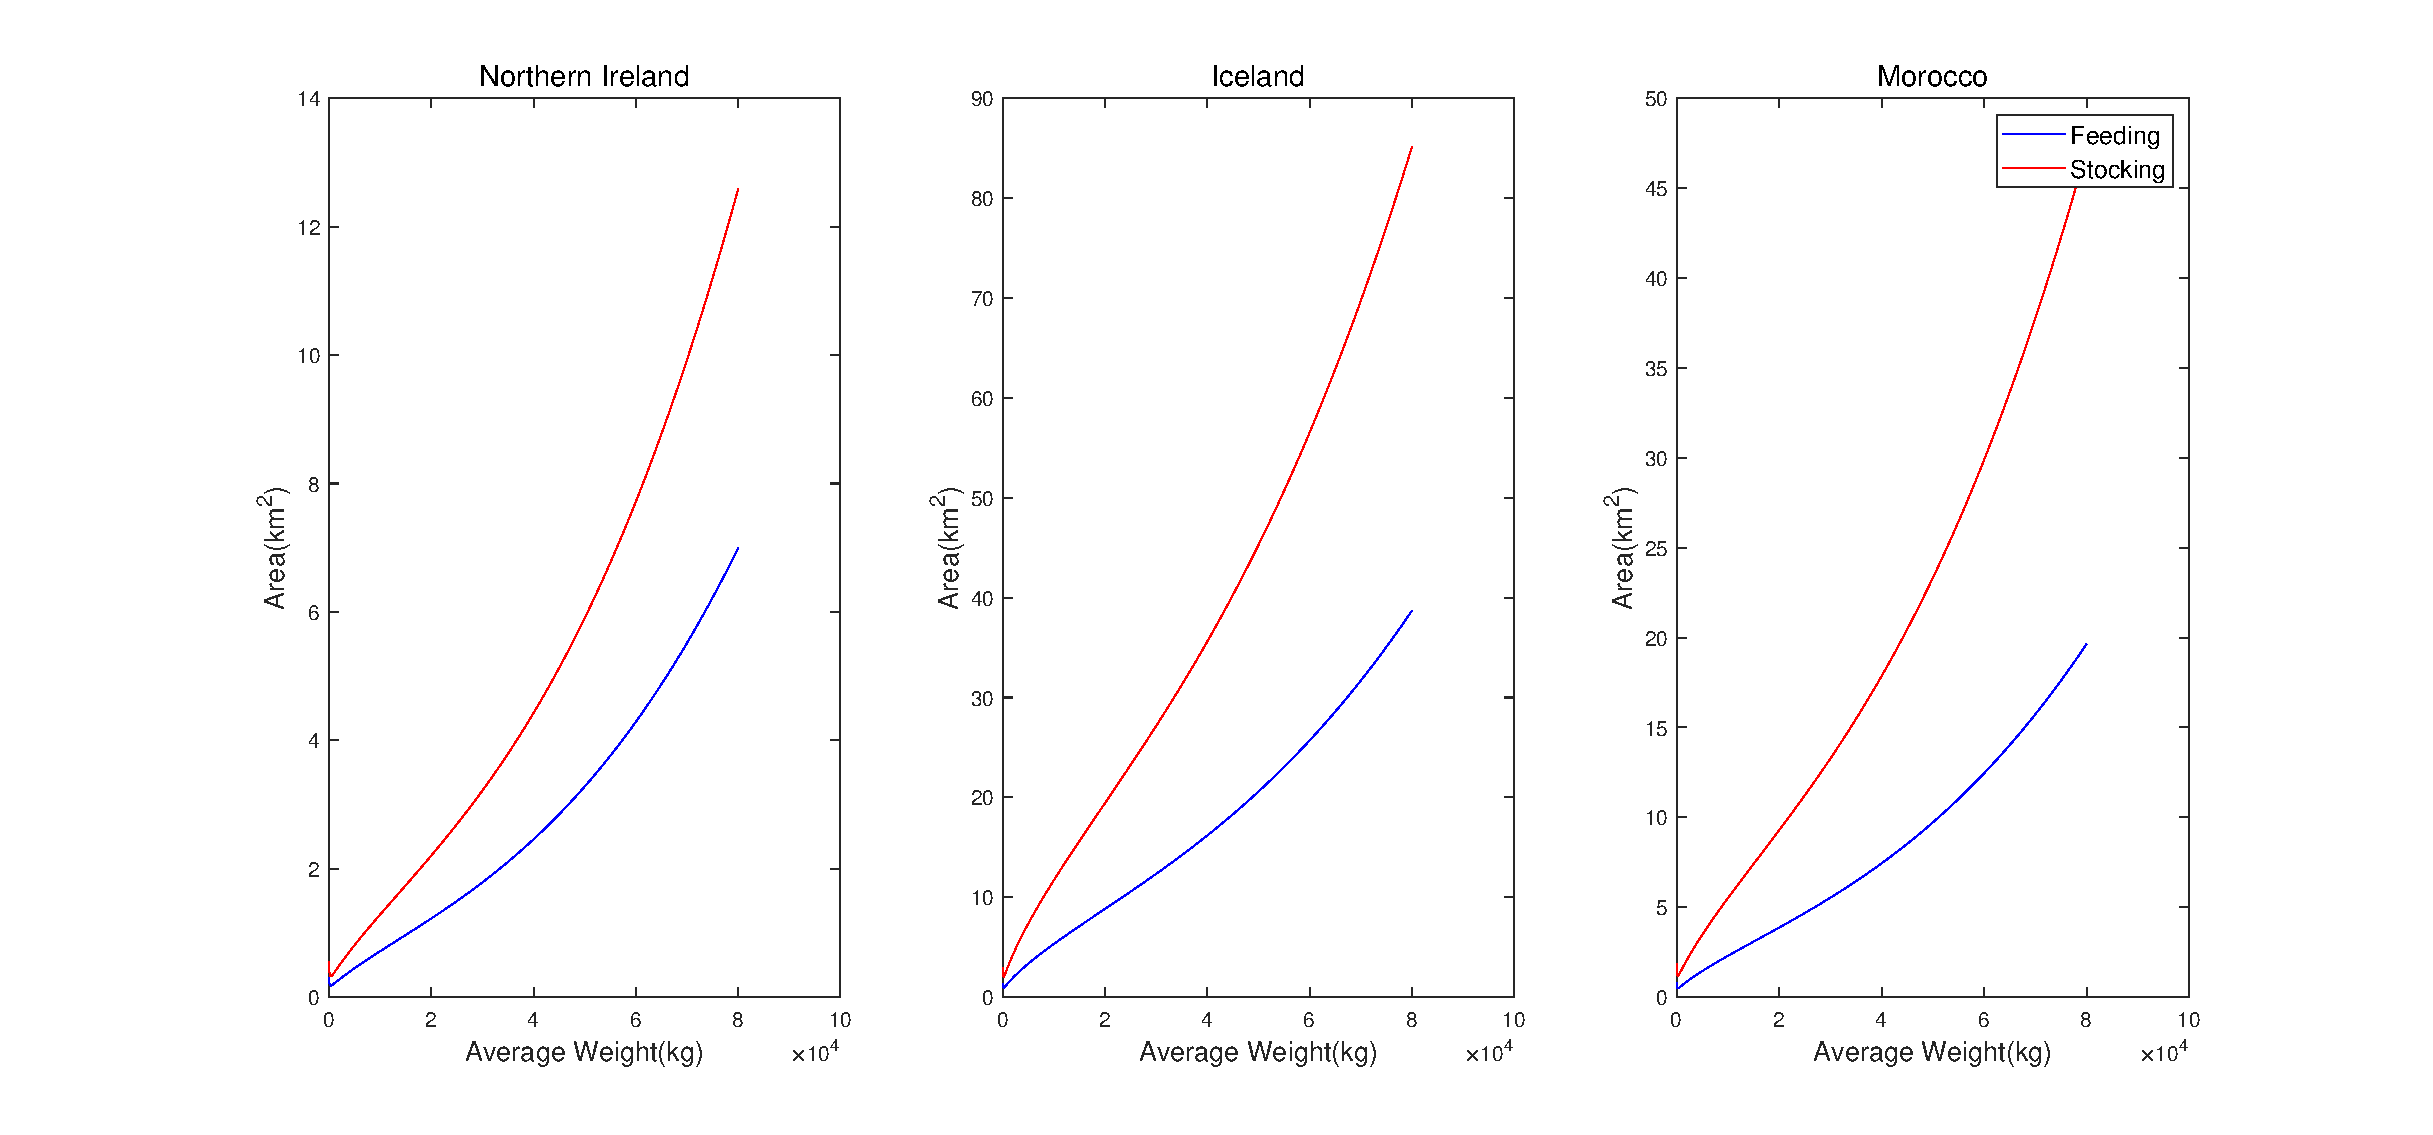
\includegraphics[width=20cm]{222.eps}}
\begin{figure}[!htbp]
    \small
    \caption{Relationship of weight and area in various regions}\label{jj}
\end{figure}
This figure stand for different climates, shows man-feed and wild-feed situations, relationship of weight and area. These figures all shows that undering the same climate, to get the same value of energy, the required area of man-feed is smaller than it of wild-feed.In another word,man-feed can get more energy than wild-feed, that means man-kind is efficient.


\subsubsection{Growing Dragon with mixed feeding}%模型
We simulate the situation of mixed feeding. Base on mentioned above, we combine total man-feed and wild-feed.

\centerline{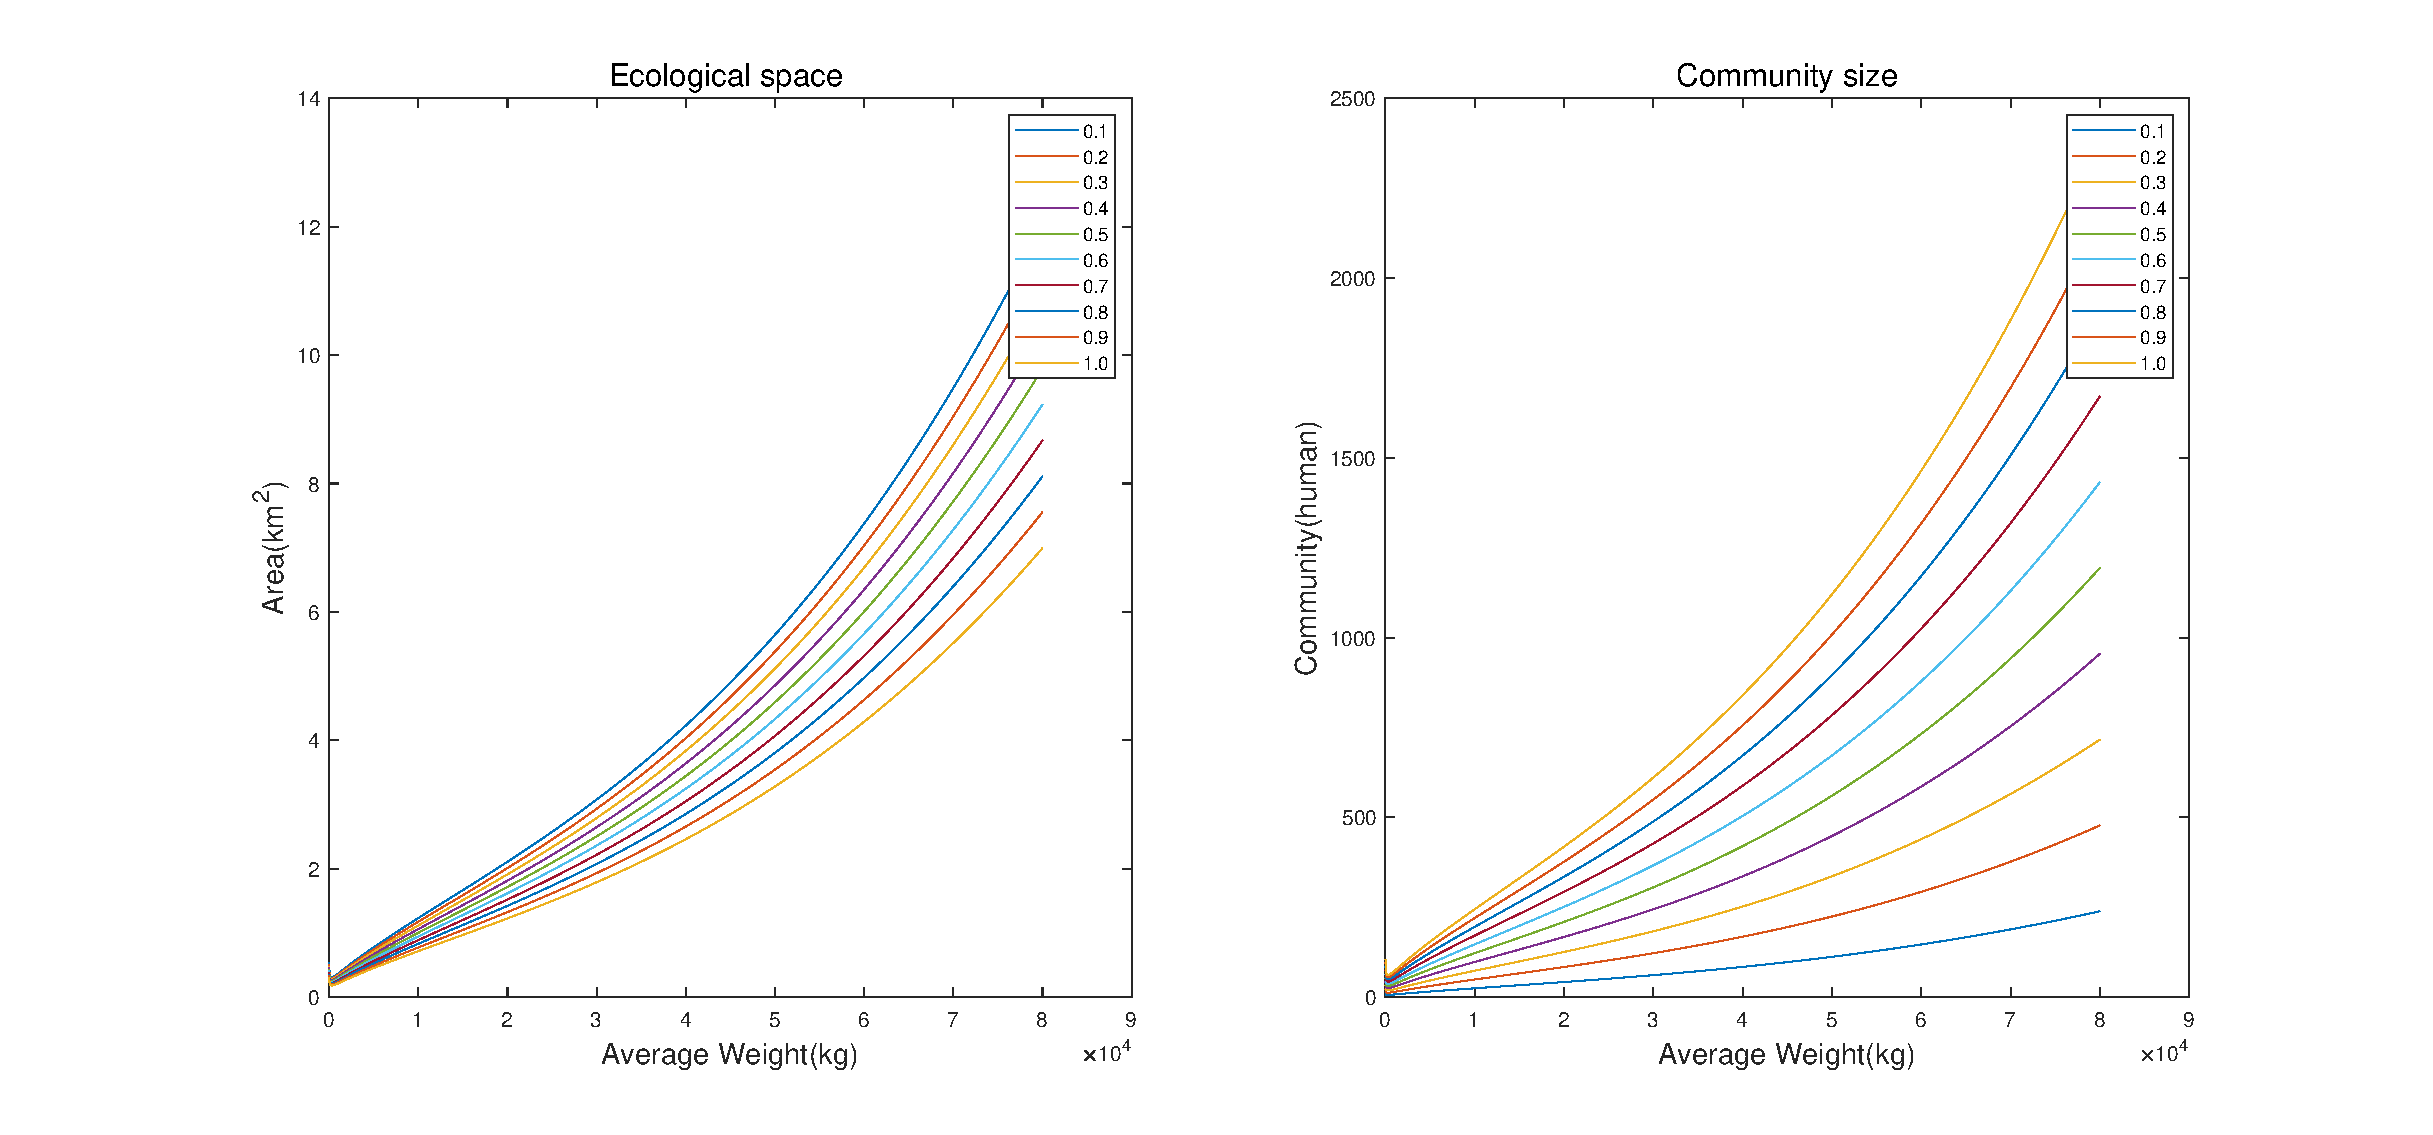
\includegraphics[width=20cm]{mix-feed.eps}} %食物链
\begin{figure}[!htbp]
    \small
    \caption{Relationship of average weight and area}\label{jj}
\end{figure}
This figure shows,undering differrent ratio of man-feed and wild-feed,the relationship of area and weight. According our figure, we can easily find: as increase of the ratio of man-feed, the weight of Dragon is increase.That means man-feed is better than whild-feed.In another word, different community have different aid to Dragon.

%%%%%%%%%优缺点
\section{Conclusion}
We build a model centering energy and associated with climate and weight of Dragon. We divided the model into two parts. One part is flight,metabolism,diet,spray fire model.Finally expressed as energy function, espcially wingspan,weight,temperature are important parament.The other part is model between energy of Dragon and ecosystem.Amount of sunlight radiation and temperature is independent variable. Combine the two parts, we build the model about energy,area,climate,weight of Dragon.

According to our model, to grow to the same weight under differrent climate need different area to feed the Dragon.In order to analysis different climate effect the Dragon easily and precise, we assume the utilization rate is 100 percent. In another word, all energy is produce to the Dragon and don't consider ecological recovery rate. In this situation, we can more intuitive cognition. Undering warm climate, required area is the least, after it is hot climate, the most is cold climate.That means, undering warm climate, the required area for rasing Dragon is the smallest. At the same time, Dragon can get the most energy, and grow biggest.That proves our assumption.

What's more, according the background in the series. Dragon growth depend on man-feed and wild-feed. We will discus how to make Dragon grow bigger in the same situation. Because of the difference of the two food-chain, the energy can be get is different too. According our figure, we can easily find: as increase of the ratio of man-feed, the weight of Dragon is increase.That means man-feed is better than whild-feed.
\subsection{Strengths}%优点
\begin{itemize}
    \item Fully considering the reality, a comprehensive analysis and modeling of the dragon.
	 \item The general formula was corrected and the results were verified by real data.
	 \item Using the intuitiveness of curve analysis, it is simple and clear to explain the interaction between the environment and the dragon.
	 \item Bold assumptions based on reality, innovative.
\end{itemize}

\subsection{Weaknesses}%缺点
\begin{itemize}
    \item The model results are generally in line with the actual situation, but there is still room for improvement.
	 \item Lack of a large amount of actual ecological data, unable to make a more accurate assessment of the ecological environment.
	 \item The basic model of the dragon can only obtain unified and true data through the method of evaluation.\\\\\\\\\\\\\\\\\\\\\\\\\\\\\\\\\\\\\\\\\\\\\\\\\\\\\\\\\\\\\\\\\\\\\\\\\\\\\\\\\\
 \end{itemize}



%%%%%%%%%引用部分
\begin{thebibliography}{99}
\addcontentsline{toc}{section}{References}  %引用部分标题("Refenrence")的重命名
%\bibitem{1}Elisa T. Lee, Oscar T. Survival Analysis in Public Health Research. \emph{Go.College of Public Health}, 1997(18):105-134.
%\bibitem{2}Wikipedia: Proportional hazards model. 2017.11.26. \texttt{\\https://en.wikipedia.org/wiki/Proportional\_{}hazards\_{}model}
\bibitem{1}Jeff Watson. The Golden Eagle Second Edition. \\ 2010, ISBN 978-1-4081-3454-2.
\bibitem{2}Dinosaurtheory: The Science of Flight and the Paradox of Flying Pterosaurs.\\ 2017.1. \texttt{\\https://dinosaurtheory.com/flight.html}
\bibitem{3}Wikipedia: Aerodynamic flight.Animal flight.\\ 2019.1.9. \texttt{\\https://en.wikipedia.org/wiki/Flight}
\bibitem{4}Kun Chen: Morphology,Flight Kinematics and Bionics of Silent Flight Owl. 2012.5.31.
\bibitem{5}James Powell : Induced Power.\\ 2002.02.15. \texttt{\\http://www.math.usu.edu/powell/ornlab-html/node7.html}
\bibitem{6}McCormick, Barnes W.: Aerodynamics, Aeronautics, and Flight Mechanics.  John Wiley \& Sons\\ 1979, ISBN 0-471-03032-5.
\bibitem{7}Tatsuo Motogawa. : Elephant Time, Mouse Time.\\2010.6, ISBN 978-7-5442-4721-4.
\bibitem{8}Mochida, Tohru: Convective and Radiative heat Transfer Coefficients for the Human Body. 1977.07.11(84):1-11.
\bibitem{9}John Latham, Renato Cumani, Ilaria Rosati and Mario Bloise : Global Land Cover SHARE (GLC-SHARE)database Beta-Release Version 1.0 - 2014
\bibitem{10}OECD Environmental Performance Reviews: Iceland 2014 \\ISBN 978-92-64-21420-0
\bibitem{11}ren HaU, PENG Shao-Lin,LU Hong-Fang:The restoration of degraded ecosystems and restoration ecology \\2004,24(8):1756~1764
\bibitem{11}Ecological thresholds: Concept, methods and research outlooks TANG Hai-Ping*, CHEN Jiao, and XUE Hai-Li  \\doi: 10.17521/cipe.2015.0090 \\\\\\\\\\\\

\end{thebibliography}

\section{Letter}

\begin{flushleft}
To: George R.R. Martin\\ 
From: Investigration Team\\
Date: 28 Januaray, 2019\\
Subject: Suggestion for\\
\end{flushleft}

Dear Martin,First of all, it's ours honor to build model about Drogon,Rhaegal,Viserion in MCM. As senior fan, I'm very glad to start my travel of raising Dragon.

We hope that in this short period of time, we will build a model with a good scientific foundation for the dragons in the play. Through various energy analysis, we can know what kind of material we need if we really raise one or more dragons. basis? Or what kind of ecological foundation should it have? How large a human community can support an adult dragon? And analyze the pressure that the dragon may cause on the ecological environment. Next we will briefly tell you about our insights.

As far as we know, Dragon isn't real in reality life, but this not hinder us doing research on them , even provide a realistic basis for the story.  In the real world, according to Aerodynamics, the bigger the body type is,the harder for the bird to fly, so Dragon can't be real. But on a land where full off magic, huge creature like Dragon is allowed to exist. So compared with eagle, Dragon have to cost more energy and power, and should have a higher ratio of wings.

So when we do research should analogy the biggest bird in the real world. Besides, we should introduce some correction factors. Finally, we build a model centering energy and associated with climate and weight of Dragon. We divided the model into two parts. One part is flight,metabolism,diet,spray fire model.Finally expressed as energy function, espcially wingspan,weight,temperature are important parament.The other part is model between energy of Dragon and ecosystem.Amount of sunlight radiation and temperature is independent variable. Combine the two parts, we build the model about energy,area,climate,weight of Dragon.

According to our model, to grow to the same weight under differrent climate need different area to feed the Dragon.In order to analysis different climate effect the Dragon easily and precise, we assume the utilization rate is 100 percent. In another word, all energy is produce to the Dragon and don't consider ecological recovery rate. In this situation, we can more intuitive cognition. Undering warm climate, required area is the least, after it is hot climate, the most is cold climate.That means, undering warm climate, the required area for rasing Dragon is the smallest. At the same time, Dragon can get the most energy, and grow biggest.That proves our assumption.

What's more, according the background in the series. Dragon growth depend on man-feed and wild-feed. We will discus how to make Dragon grow bigger in the same situation. Because of the difference of the two food-chain, the energy can be get is different too. According our figure, we can easily find: as increase of the ratio of man-feed, the weight of Dragon is increase.That means man-feed is better than whild-feed.

Last but not least, our advise to these three regions is: 1.make sure to let Dragon stay at warm area to reduce metabolism. 2.increase the place to hold a Dragon. 3.increase the ratio of man-feed or improve the diet structure to make Dragon get much more energy,and reduce loss. That's a good way to make Dragon grow fast.

Our model considers the most significant factors.Thus, we hold this model to be a useful tool.
We believe our model is useful for growth of Dragon. You’re welcome to contact us at any time for more communicate.


\end{document}

%%%%垃圾箱

 	 % \centerline{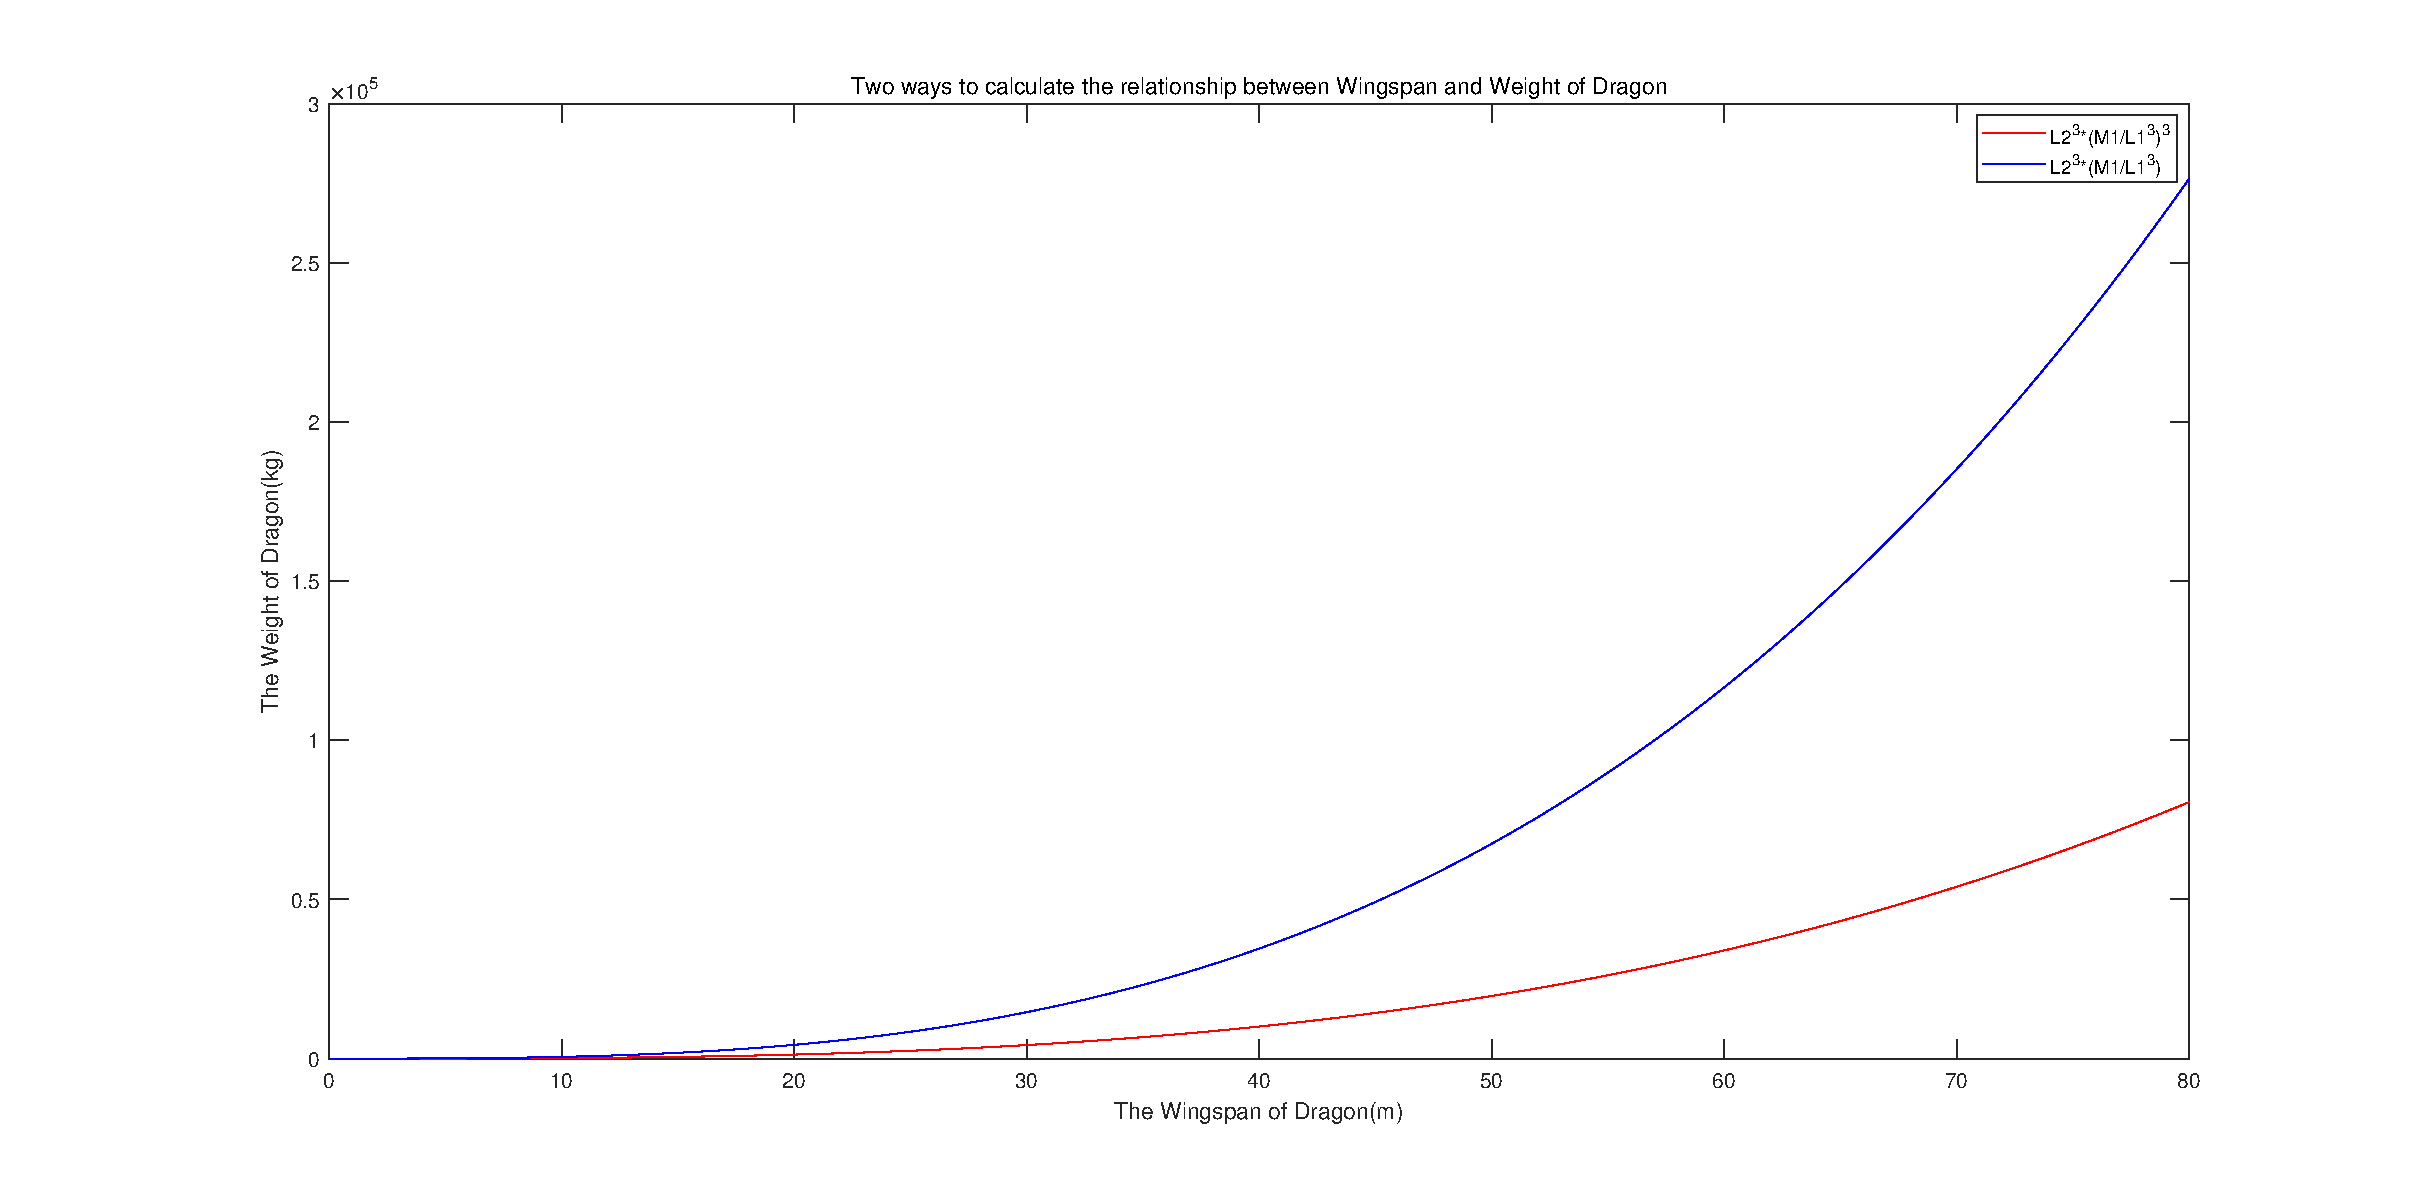
\includegraphics[width=20cm]{Two-ways-to-calculate-the-relationship-between-Wingspan-and-Weight-of-Dragon0.eps}}%两种计算方法对比图

%\begin{figure}[!htbp]
%    \small
%    \caption{Two ways to calculate the relationship between Wingspan and Weight of Dragon}\label{jj}
%\end{figure}

\subsubsection{shit}

\centerline{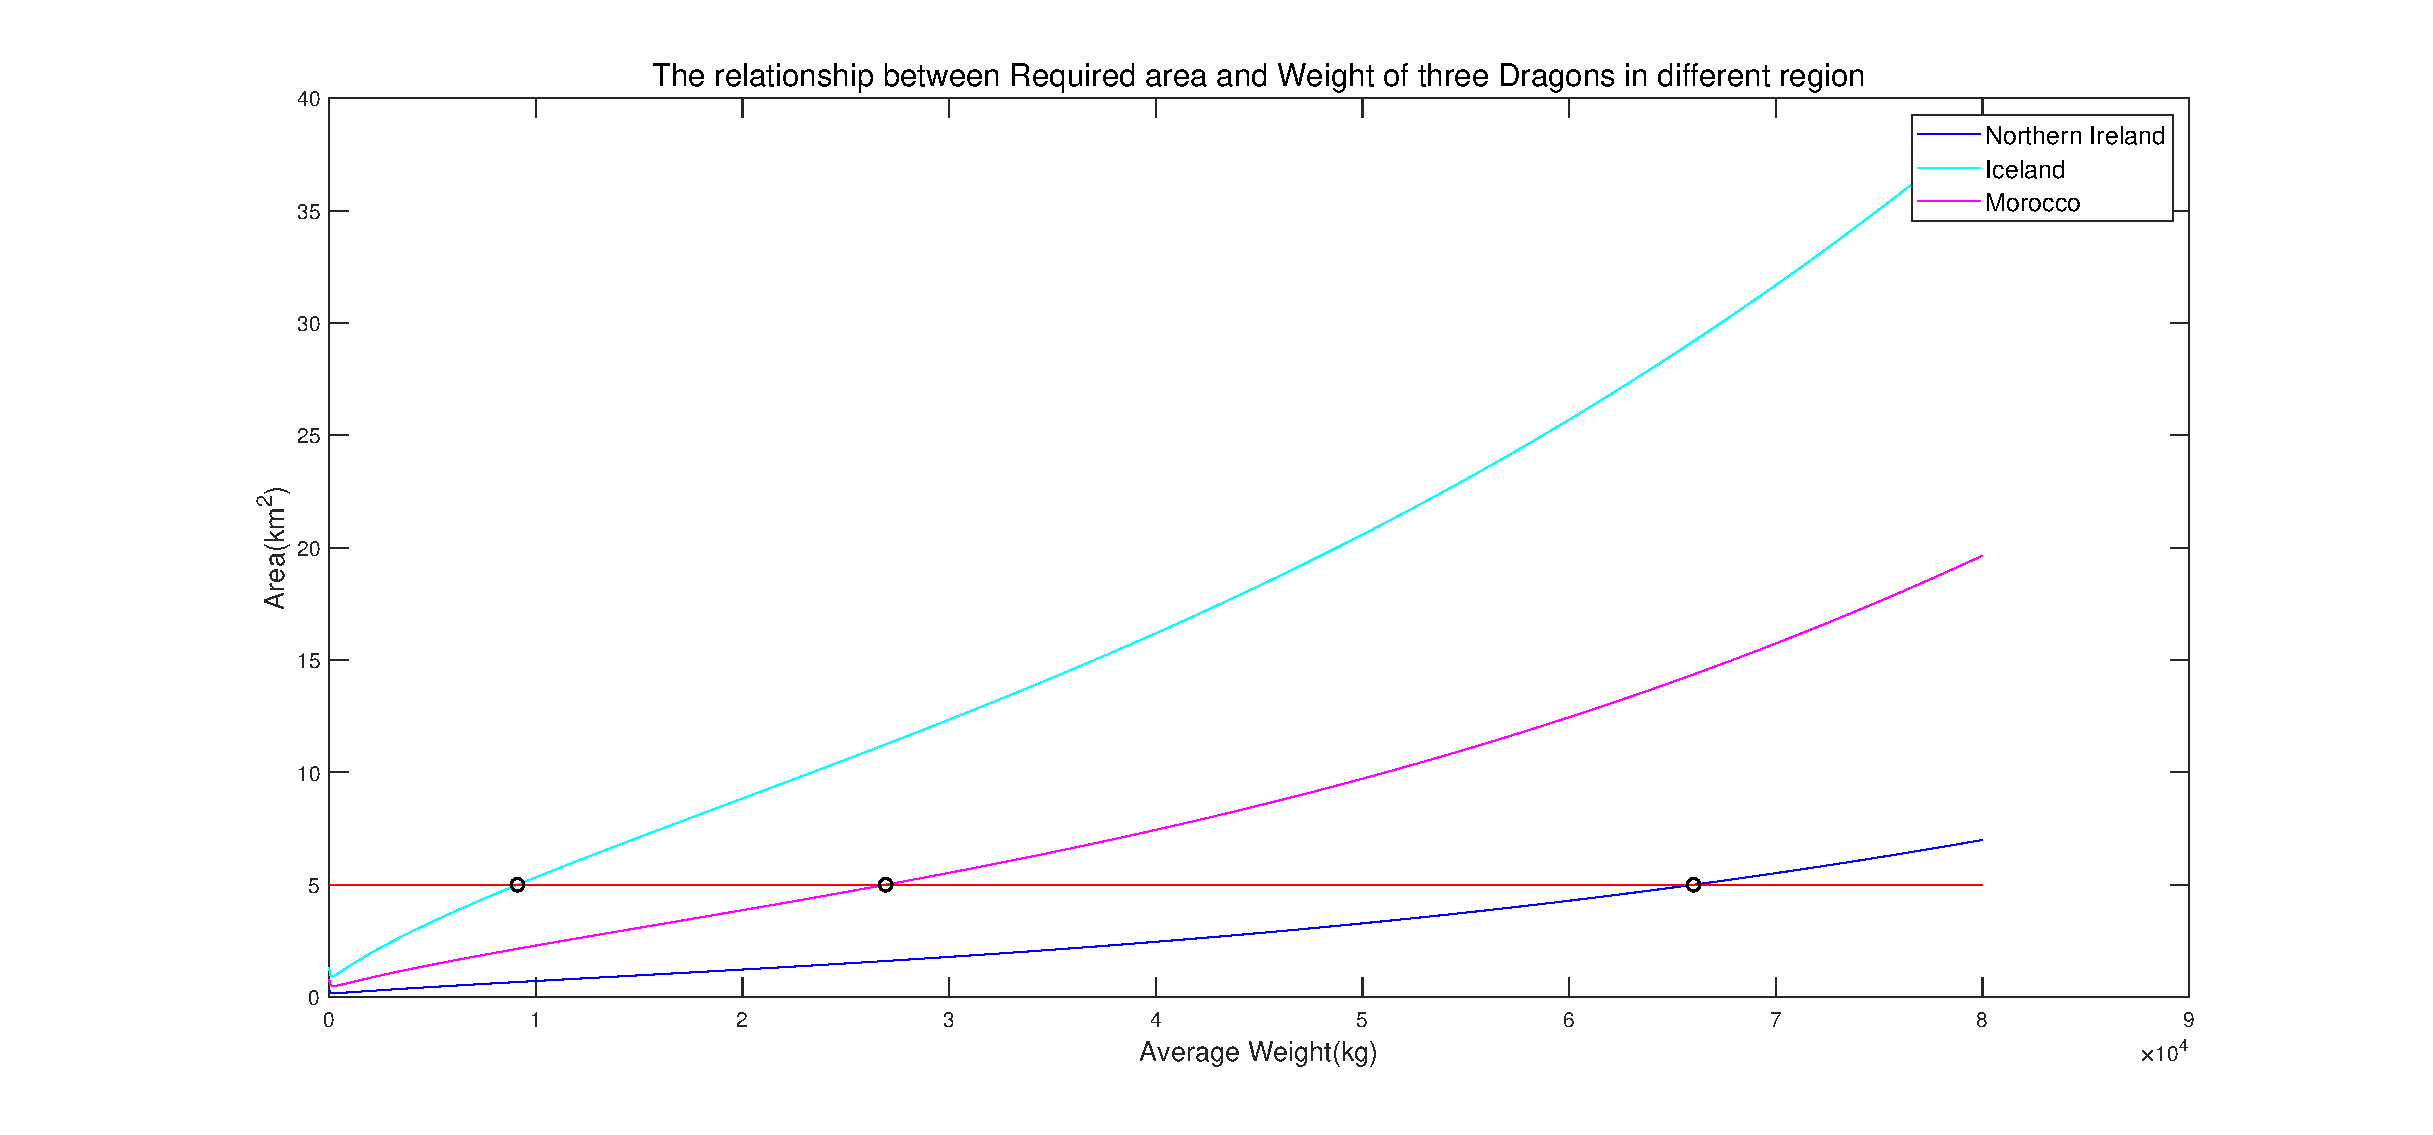
\includegraphics[width=20cm]{areagd1.eps}}
\centerline{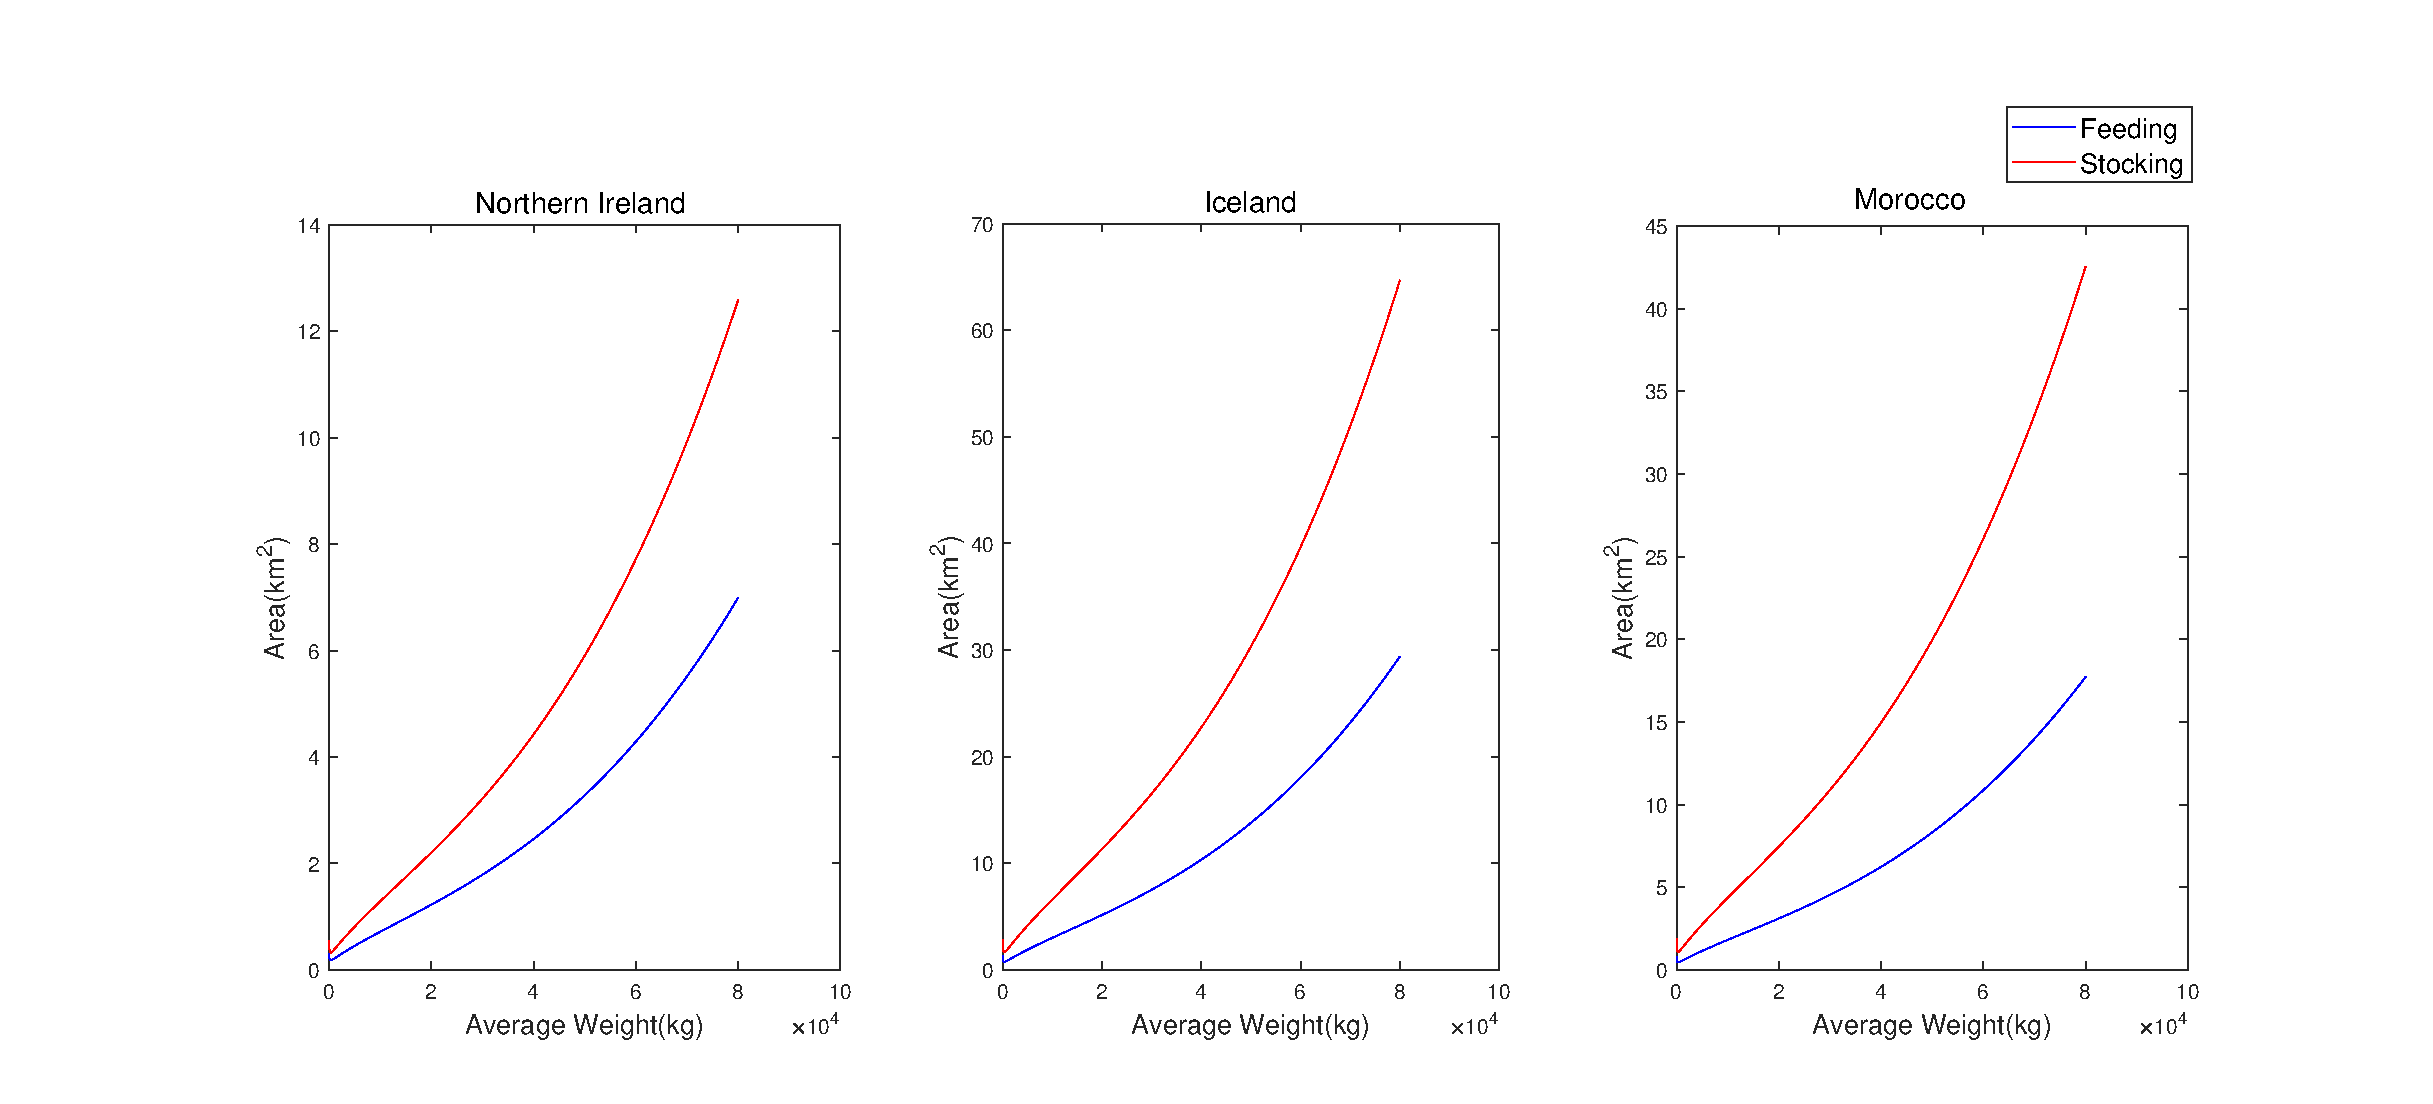
\includegraphics[width=20cm]{Different-ways-of-raising-dragons.eps}}
\centerline{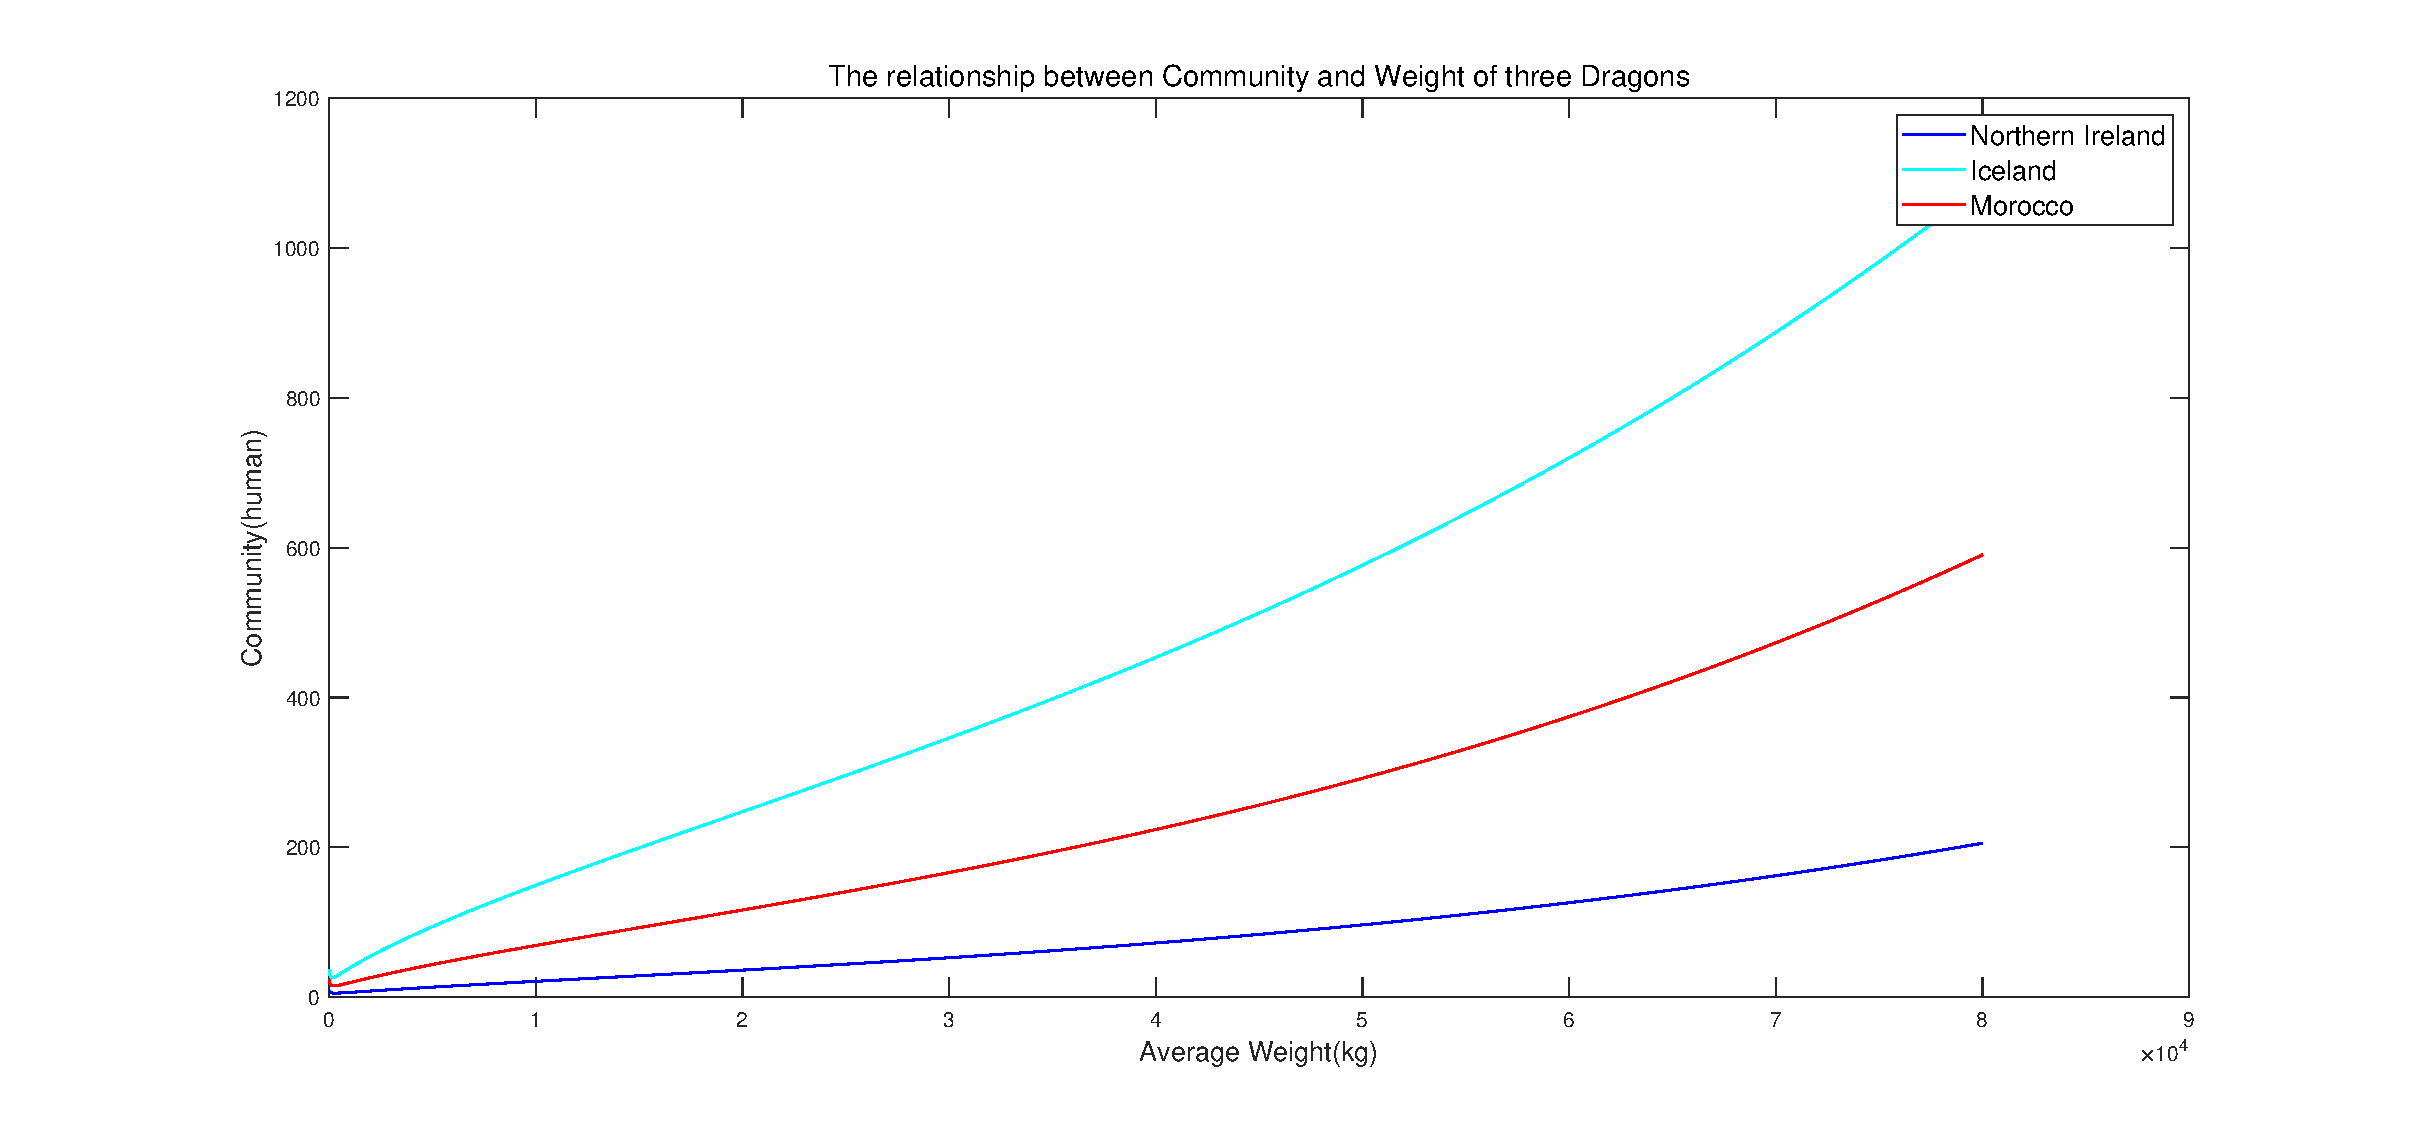
\includegraphics[width=20cm]{The-relationship-between-Community-and-Weight-of-three-Dragons.eps}}%社区与三龙的体重
\centerline{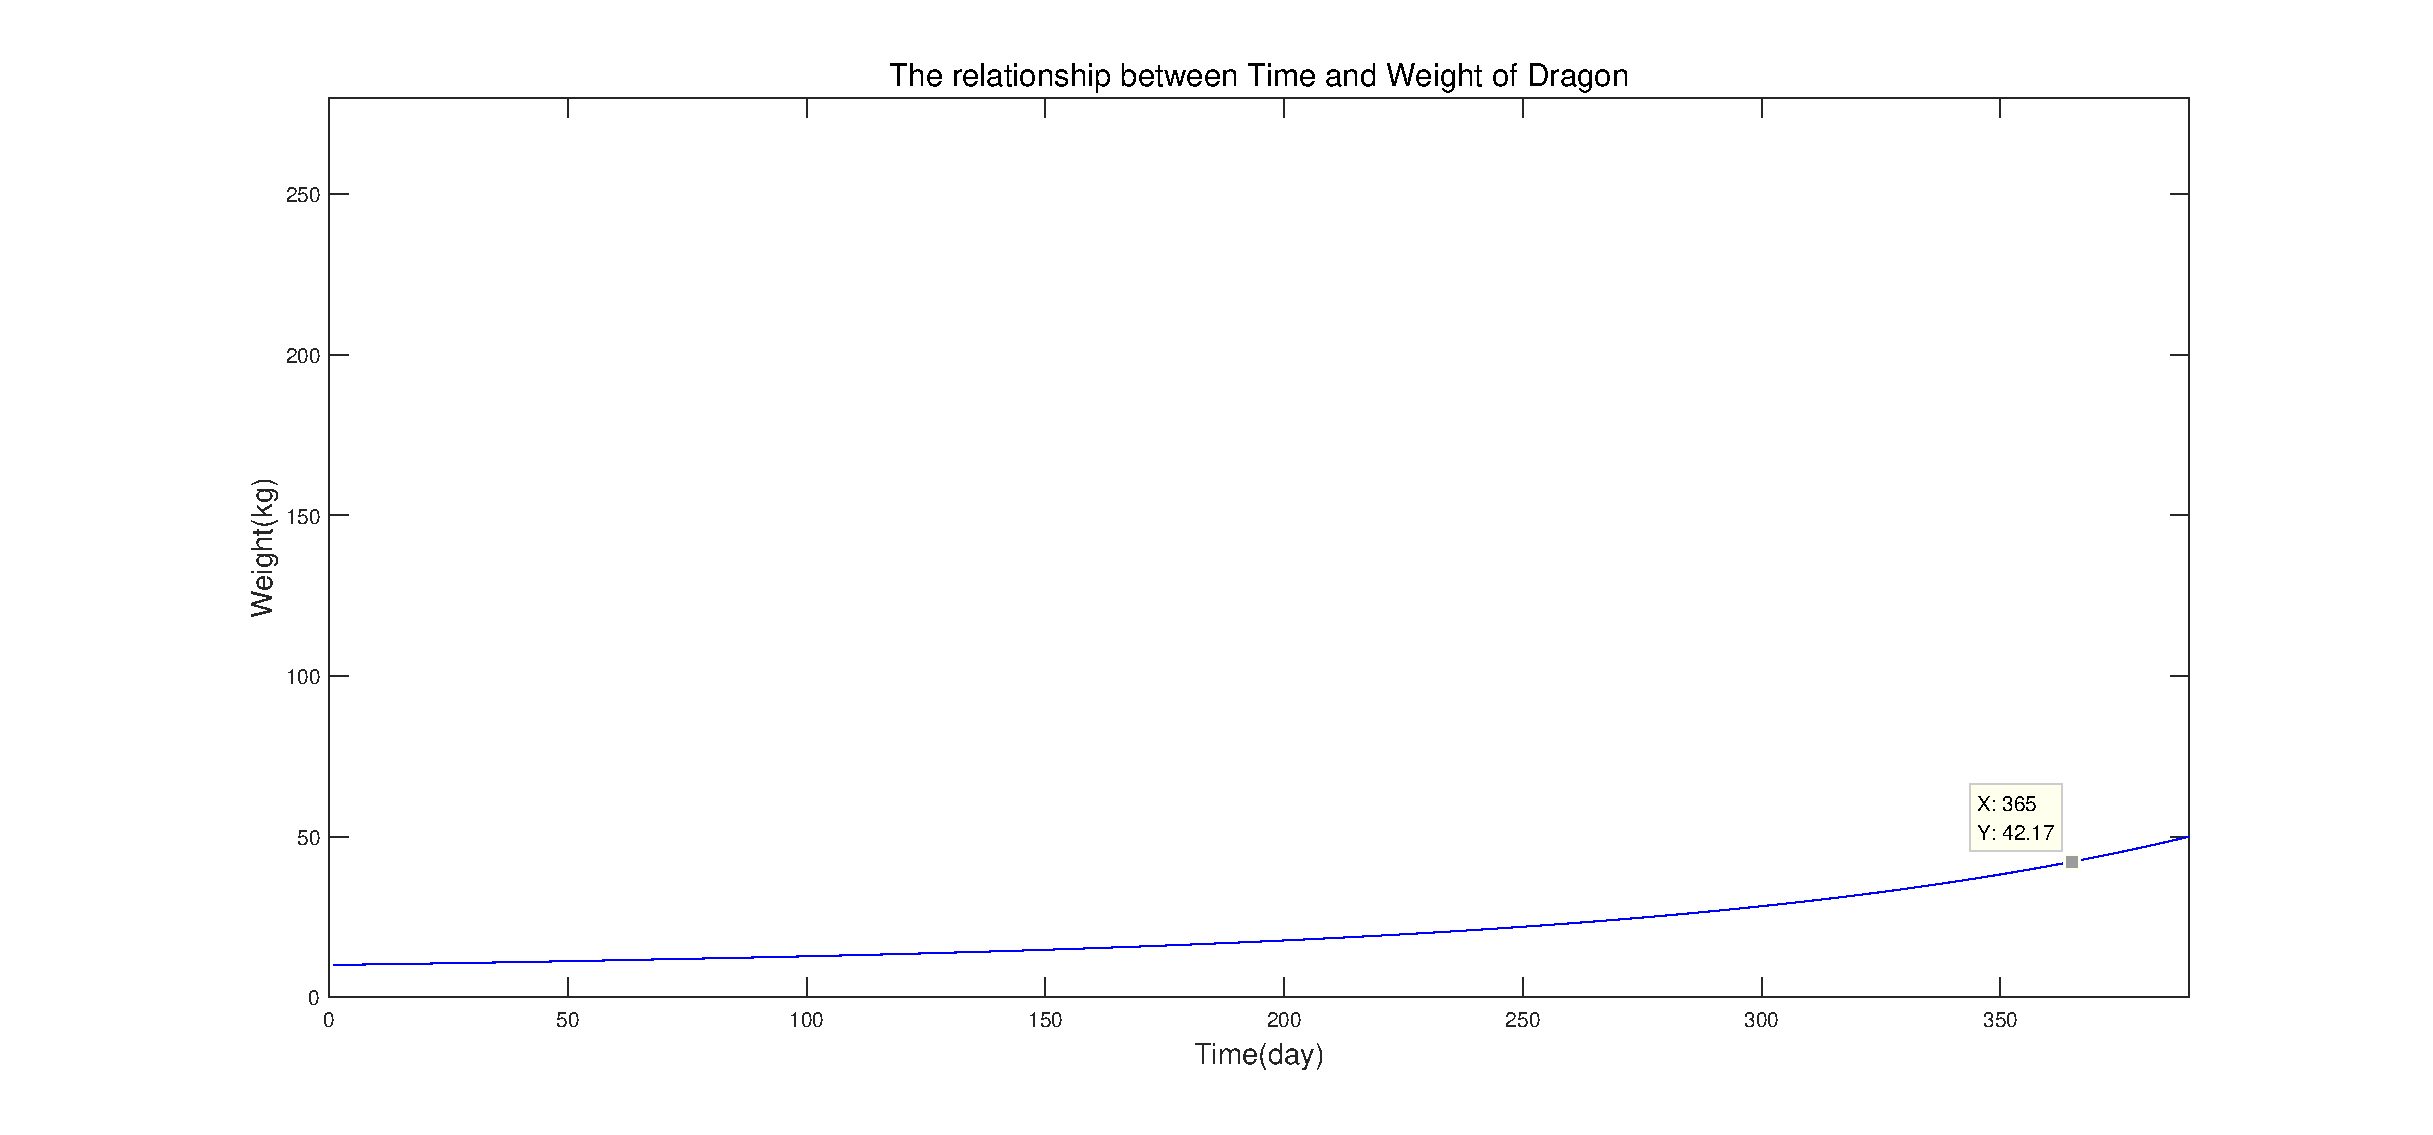
\includegraphics[width=20cm]{grow1.eps}}

